\section{extrasolar: todo}

\begin{wordonframe}{Osservazioni: Da ''Physical properties of extrasolar planets''}\tolbf
\begin{itemize}
\item Observed properties: ralation host star metallicity-frequency pf planets, large radius of transiting planets; pg 42 radius anomaly, brown dwarf vs massive planets, Hot Neptune (link to seminario?), light from exoplanets.
\item Interior structure: pg13 EOS composition, Earth-super Earth and Neptune-Super jupiter (18-19); Evolution (pg 30)
\end{itemize}
\end{wordonframe}

\begin{wordonframe}{Udry 03:I, II}
constrain on migration scenario: runaway migration
\end{wordonframe}

\begin{wordonframe}{ridefinisco sezioni}
\begin{itemize}
\item Campagne osservative, effetti di selezione e risultati: Transiti e RV. Udru Santos 07, Winn Fabrycky 15.
RV: mayor11, Howard 10, Moutou13,
T: coughlin16, petigura 13, fressin 13,howard 12
ML: cassan 12
DI: bowler 16
\item Relazioni sistemi planetarii propriet\'a stellari.
CK-survey 4: Metal-rich stars host greater diversity of planets; giant planet occurrence in stellar mass-metallicity plane; planet populations as a function of stellar properties; cumming 08
\item 
\end{itemize}

\end{wordonframe}

\section{Osservazioni}

\begin{comment}
\begin{frame}{caratteristiche alcuni sistemi extra-solari}
\begin{table}[!ht]
\pgfplotstabletypeset[col sep=comma,skip rows between index={4}{10},
every head row/.style={
 %before row={},
 %every last row/.style={after row=\bottomrule},
 after row={\midrule}
},
%every 2 row/.style={after row=\midrule},
%every last row/.style={after row=\bottomrule},
%every first column/.style={column type/.add={|}{}},
%every last column/.style={column type/.add={}{|}},
%columns/0/.style = {column type/.add={|}{}},
%columns/5/.style = {column type/.add={|}{}},
%columns/0/.style={string type},
display columns/0/.style={column name={number},clear infinite},
%display columns/2/.style={column name={e},clear infinite},
%display columns/3/.style={column name={i},clear infinite},
%display columns/4/.style={column name={$\tau_{sid}$},clear infinite},
%display columns/5/.style={column name={obliquity},clear infinite},
%display columns/planets/.style={column name={pianeta},string type},
%create on use/planets/.style={create col/set list={Mercury, Venus, Earth, Mars,Jupiter,Saturn,Uranus, Neptune}},
%columns/planets/.style={string type},
columns={numname},
%columns={planets, dps, e, i, Ps, obl},
/pgf/number format/precision=3
     ]{exoplanets.csv}
\end{table}
\end{frame}
\end{comment}

\begin{wordonframe}{extrasolar: problemi aperti}
Distinzione pianeta/brown dwarf: $M_P\leq20M_J$, i pianeti veri e propri hanno masse $M_P\leq13M_J$.
Domande fondamentali:
\begin{itemize}
    \item Quanto \'e frequente la formazione di sistemi planetari all'atto di formazione stellare?
    \item Quanto \'e frequente la formazione di pianeti terrestri?
    \item Quanto \'e frequente la nascita della vita?
\end{itemize}
\end{wordonframe}

\begin{frame}[allowframebreaks]{Survey}
\begin{columns}[T]\begin{column}{0.5\textwidth}
\begin{block}{RV}
\begin{itemize}
\item Keck: Cumming 08 ($P<2000d$, $m>0.3\mjupiter$) - Keck and Lick: Howard 10
\item California planet survey (exoplanets.org)
\item HARPS (mayor 11)
\end{itemize}
\end{block}
\end{column}\begin{column}{0.5\textwidth}
\begin{itemize}
\item Corot (Moutou 13)
\item Kepler (kelper-california survey II, III, V, planet occurrence within 0.25 AU, taloe of evaporation): Coughlin 16
\end{itemize}
\end{column}\end{columns}
\begin{itemize}
\item Direct imaging: Bowler 16.
\item Microlensing: cassan 12
\end{itemize}
\begin{block}{Exoplanets catalog}
\begin{itemize}
\item Extrasolar planet encyclopedia: exoplanet.eu
\item Keck, lick, Anglo-Australian telescope: exoplanets.org
\item www.inscience.ch/transits: transit references
nsted.ipac.caltech.edu: nasa planet finding and characterization activities 
\end{itemize}
\end{block}
\end{frame}

\section{Properties of radial velocity exoplanets}\linkdest{exoRV}
%
\begin{wordonframe}{Revs about stat properties of rv exo}
Udry 03, Udry Santos 07, Santos 08, Johnson 09, Mayor 11 Winn Fabrycky 15, Cumming 14
\end{wordonframe}

\begin{frame}{Fraction of stars with orbiting planets. Detectability in M-P diagram.}

\begin{figure}[!ht]
\begin{subfigure}[b]{0.47\textwidth}
\centering
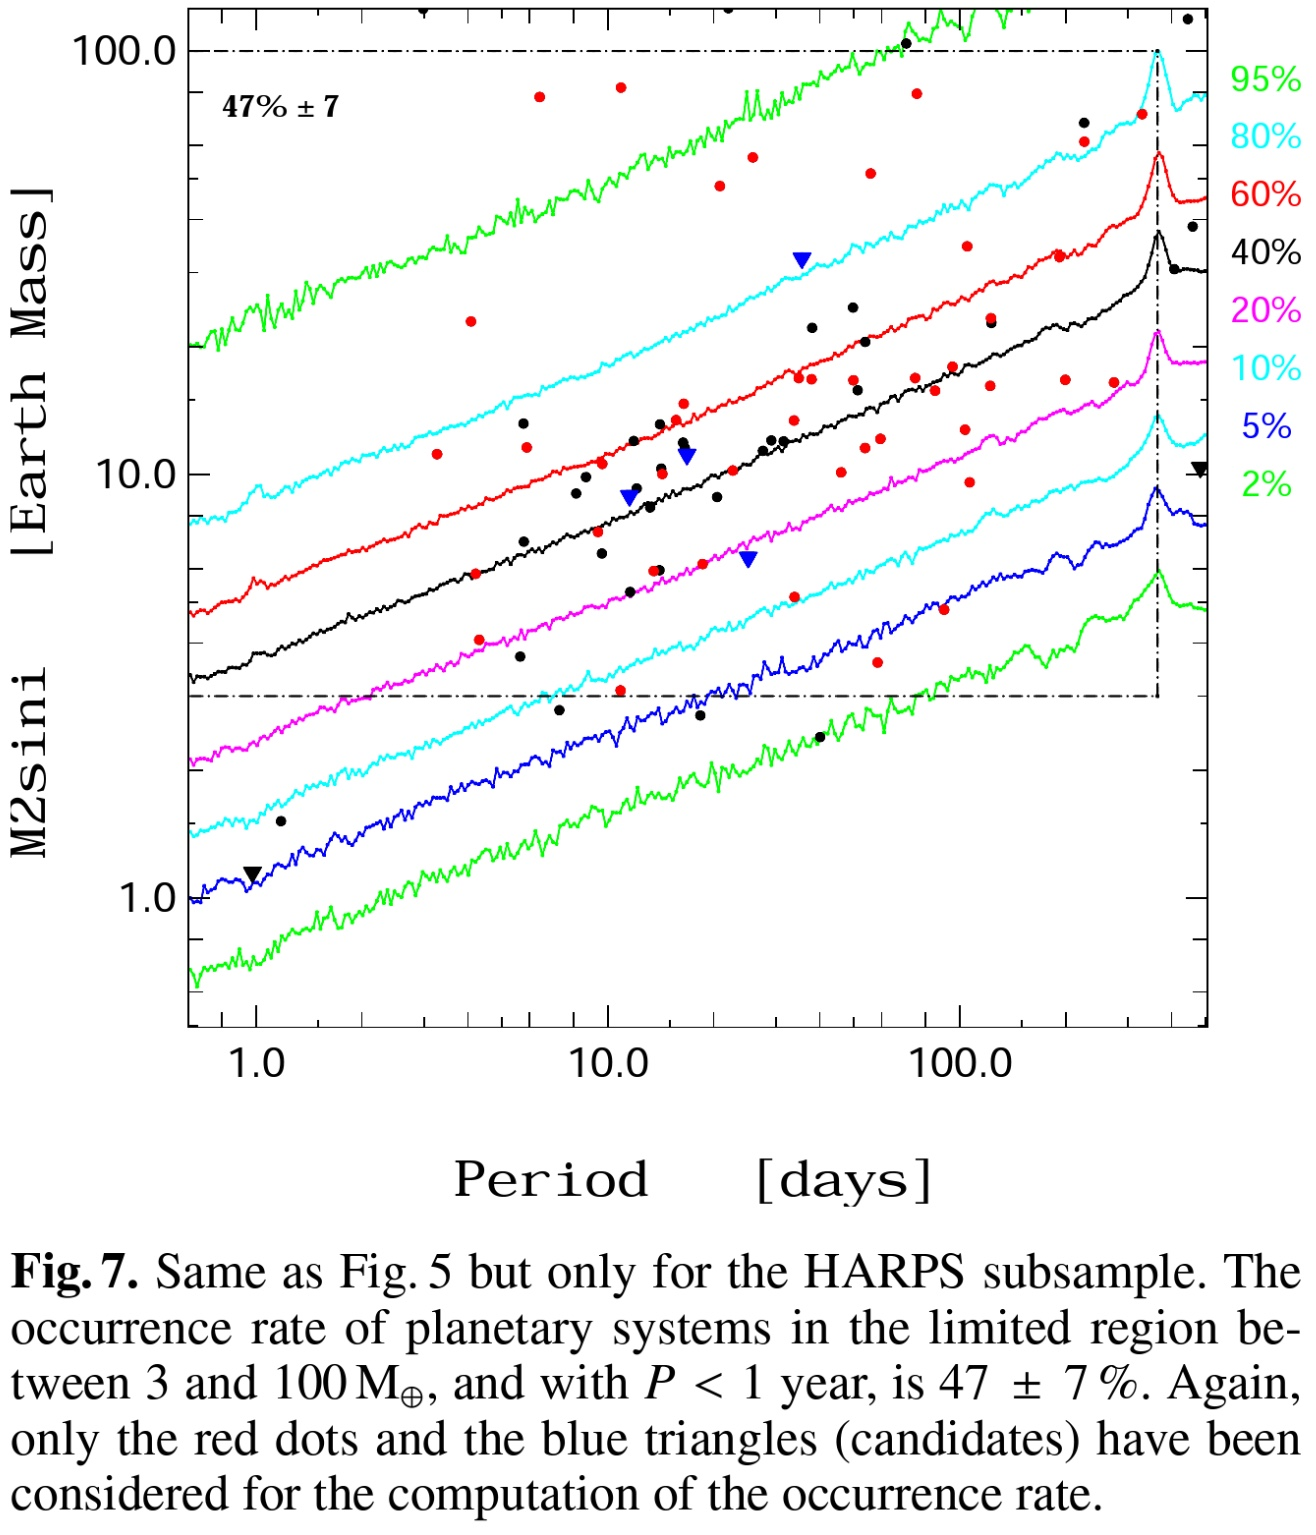
\includegraphics[trim={0cm 0 1 0},clip, keepaspectratio, height=0.4\textheight]{PMfreq-e12}
\label{fig:PMfreq-e12}
\end{subfigure} 
~
\begin{subfigure}[b]{0.47\textwidth}
\centering
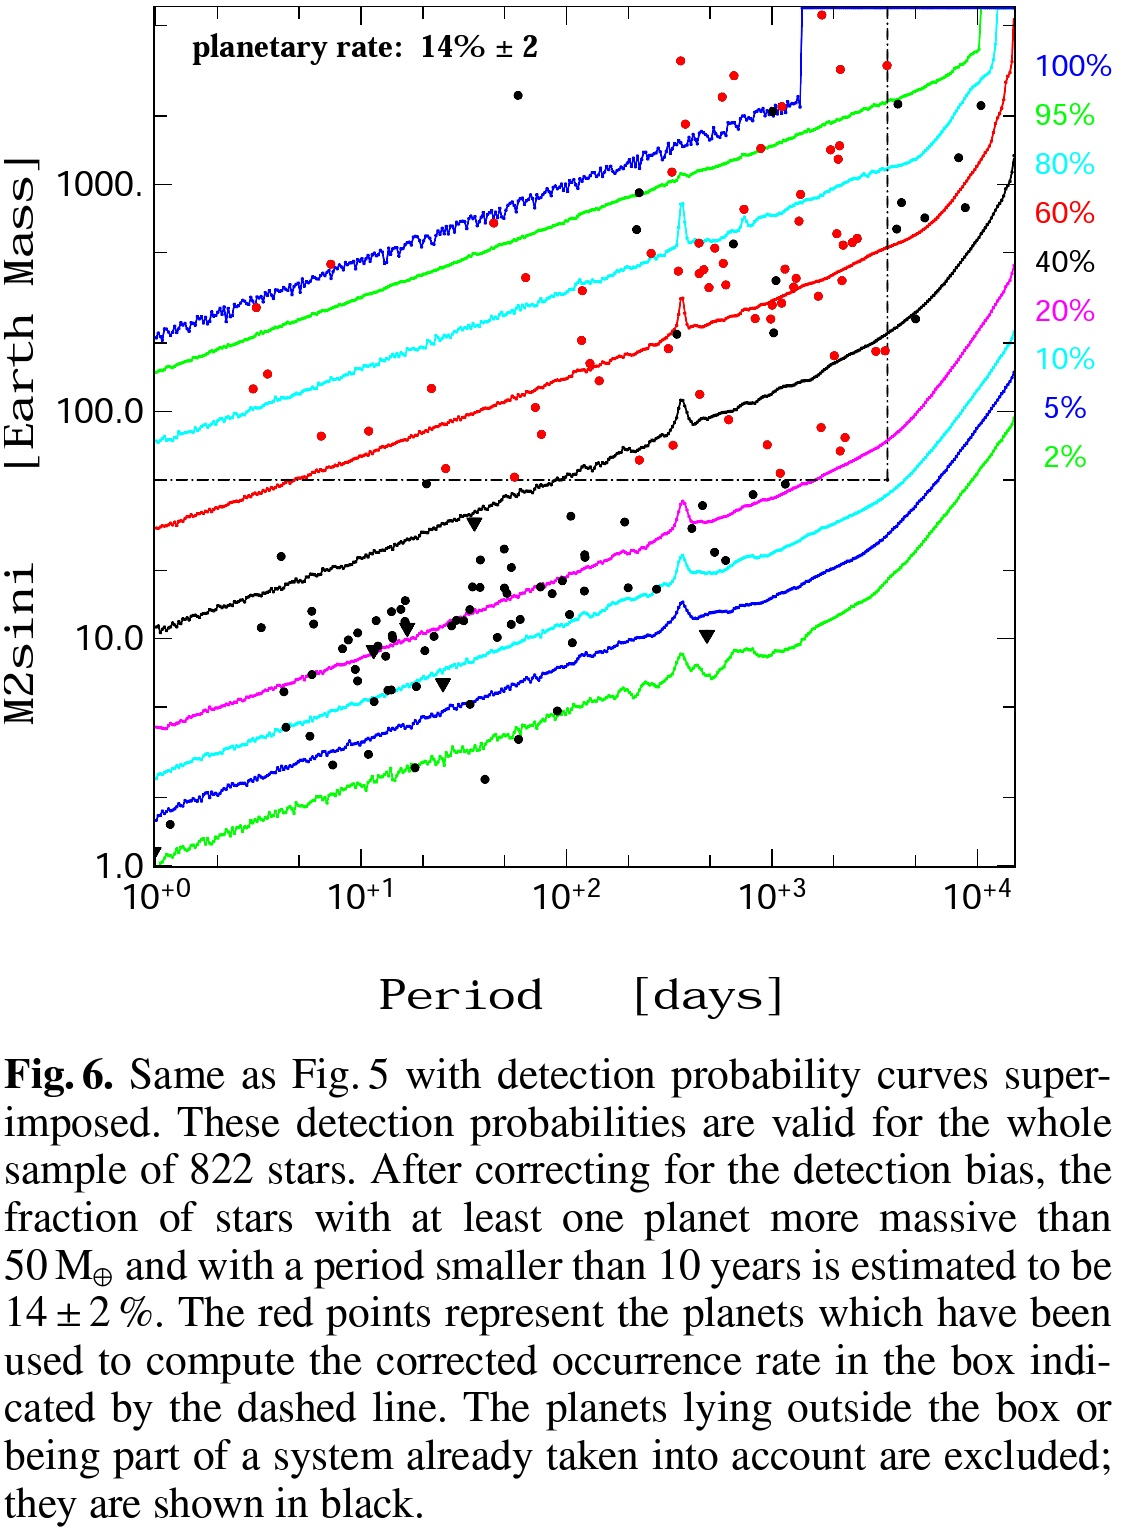
\includegraphics[trim={0cm 0 1 0},clip, keepaspectratio, height=0.4\textheight]{PMfreq-e23}
\label{fig:PMfreq-e23}
\end{subfigure}

\end{figure} 

\begin{figure}[!ht]
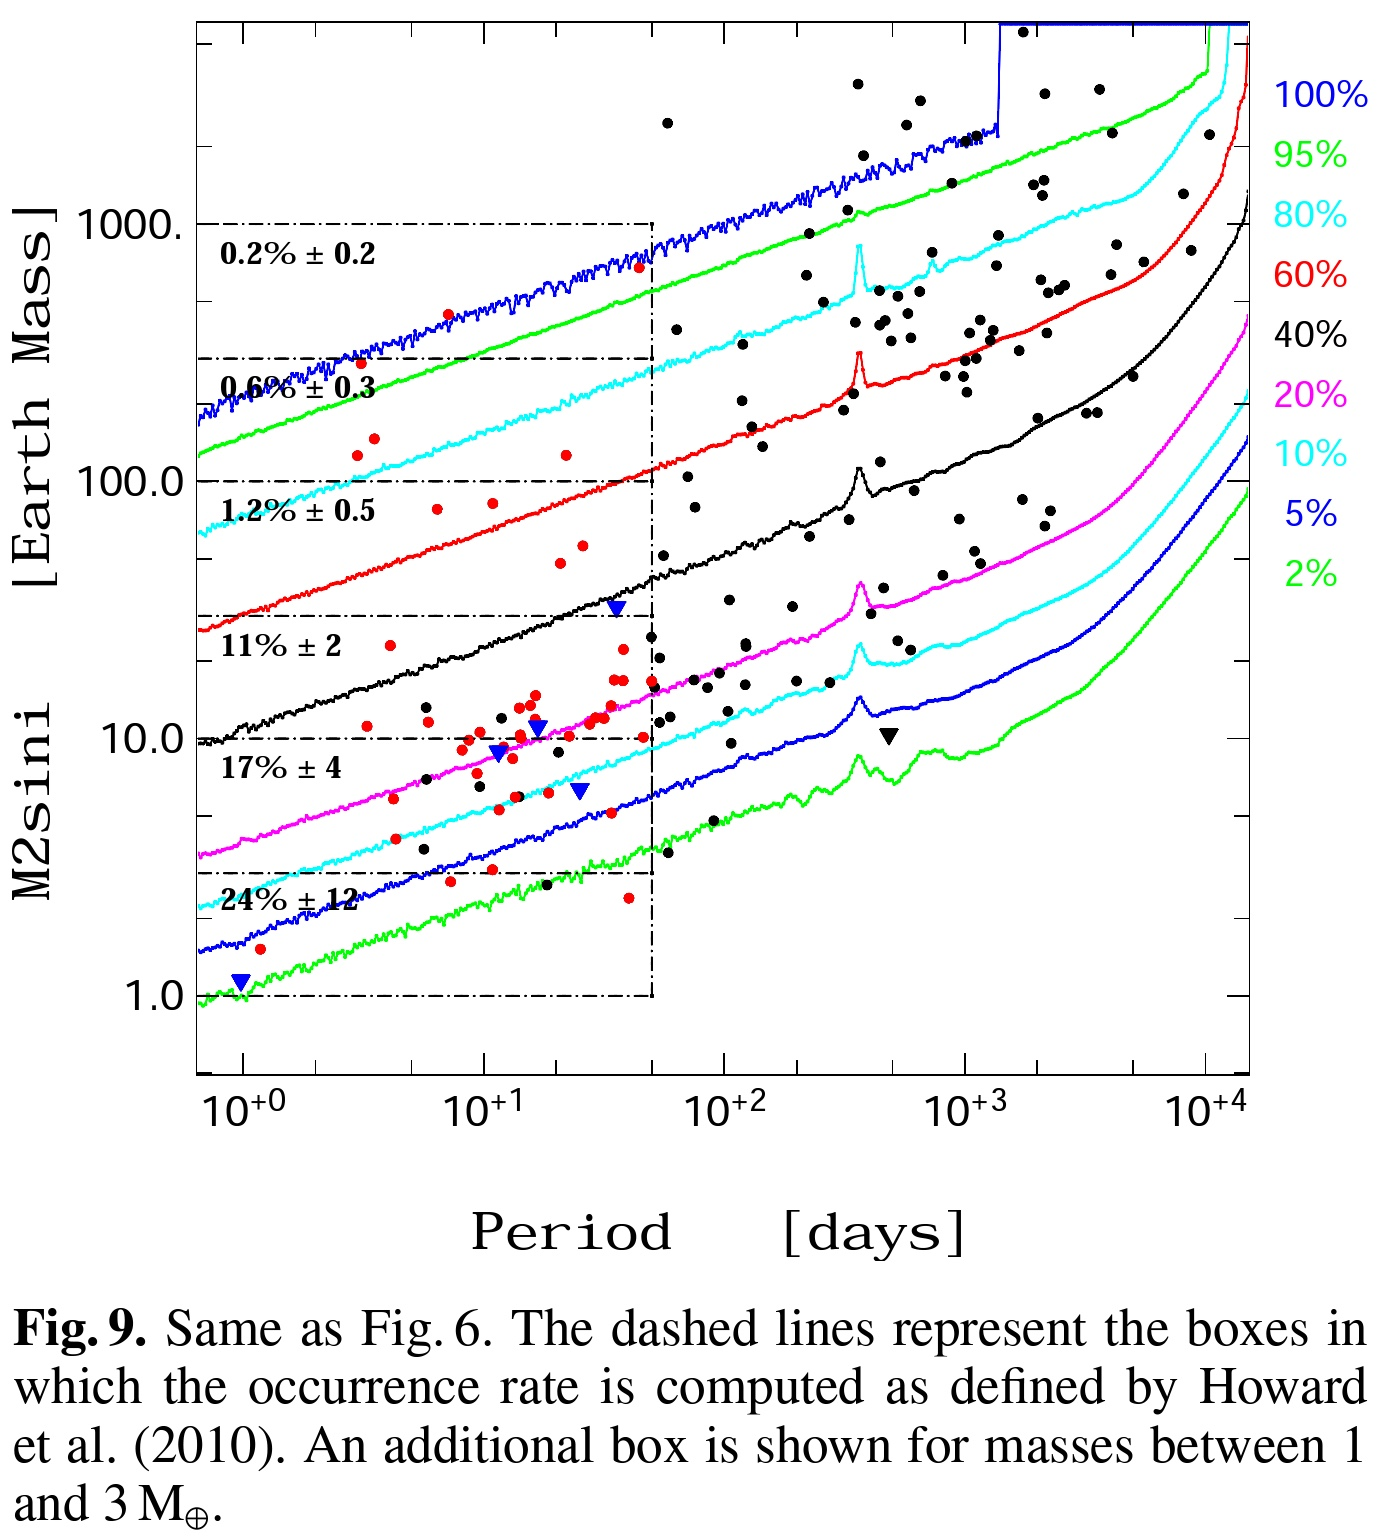
\includegraphics[trim={0cm 0cm 1 0},clip, keepaspectratio,height=0.4\textheight]{PMfreqshort}
\label{fig:PMfreqshort}
\end{figure}

\end{frame}

\begin{wordonframe}{Distribuzioni pianeti osservati tramite RV e completezza survey nello spazio dei parametri M-P}
Le linee colorate nel diagramma massa-periodo delimitano regioni al di sotto delle quali la percentuale indicata ($C(M\sin{i},P)$) di stelle ha $99\%$ di probabilit\'a di rilevamento per un pianeta in quella regione del diagramma.
Il $47\%$ di stelle ospita un pianeta nel range di massa $2\mearth{}-50\mearth{}$ delle super-terre e pianeti gioviani entro $100\mearth{}$, il $14\%$ ha pianeti gioviani ($M_p>50\mearth{}$), il $24\%$, $17\%$ e $11\%$ risp. hanno pianeta terrestre, super-terra e nettuniano con periodo entro $50d$.

$f_{pl}=\frac{1}{N_*}\sum_iN_{ij}$, $N_{ij}=\frac{1}{C(m\sin{i},P)}$ per pianeta i attorno a stella j.
\end{wordonframe}

\begin{frame}{Mass-Period distribution}
\begin{itemize}
\item \cite{marcy2008exoplanet}: Pianeti nel range di massa $0.1-12\mjupiter$ hanno distribuzione di massa $\TDy{M}{N}\propto M\expy{-1.15}$.
\item \cite{cumming2008keck}: nell'intervallo $M=0.3-10\mjupiter{}$ e $P=2-2000\si{\day}$ la distribuzione dei pianeti nel diagramma M-P segue $dn\propto M\expy{\alpha}P\expy{\beta}\,d\log{M}d\log{P}$ con $\alpha=-0.31\pm0.2$, $\beta=0.26\pm0.1$.
\item \cite{mayor2011harps}: $P<\SI{100}{d}$ dominano super-terre e pianeti nettuniani, shortage of massive planets at short periods ($0.5-1\%$ Hot Jupiters), frequency of gaseus giant planets strongly increasing with $\log{P}$, lack of light planet ($M<0.75\mjupiter{}$) on periods larger than \SI{100}{day}.
\end{itemize}
\end{frame}

\begin{frame}{Distribuzione di massa planetaria: RV, Mayor 11}
\begin{figure}[!ht] \begin{subfigure}[b]{0.47\textwidth}
\centering 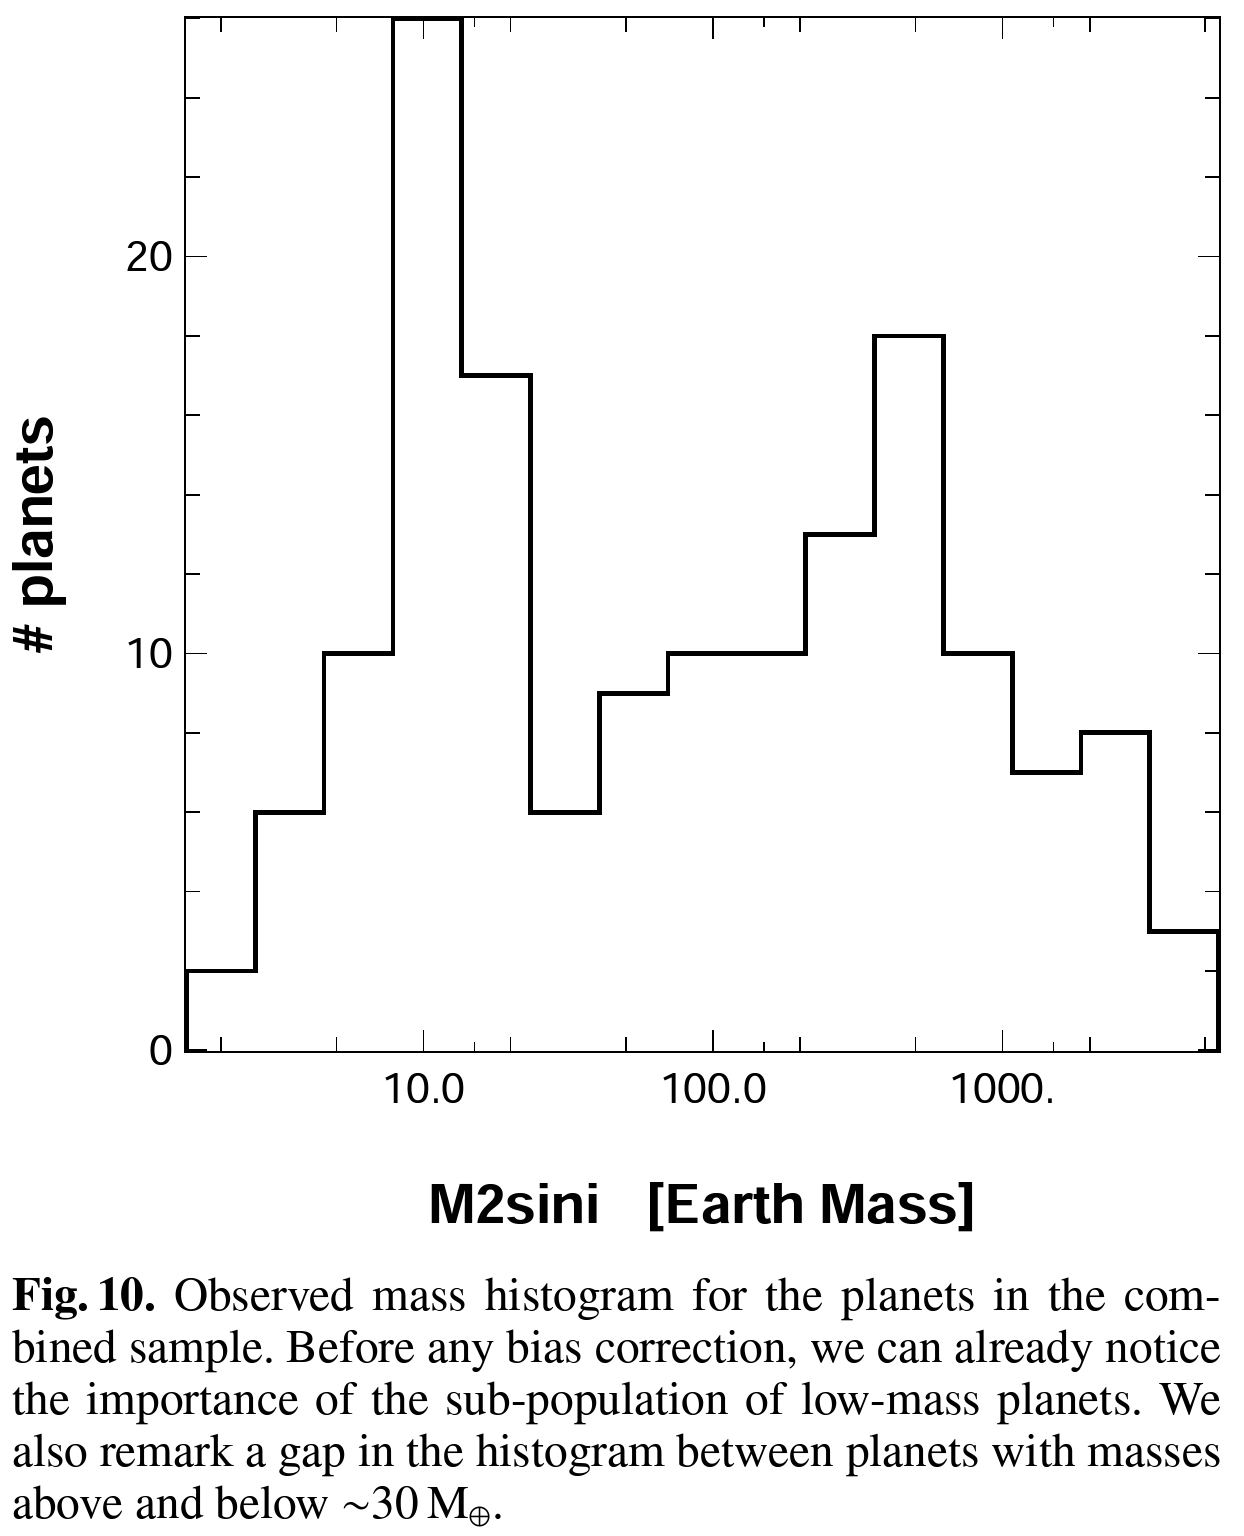
\includegraphics[trim={0cm 0 0 0},clip, height=0.45\textheight]{pvsM} \label{fig:pvsM} \end{subfigure}
~
\begin{subfigure}[b]{0.47\textwidth} \centering 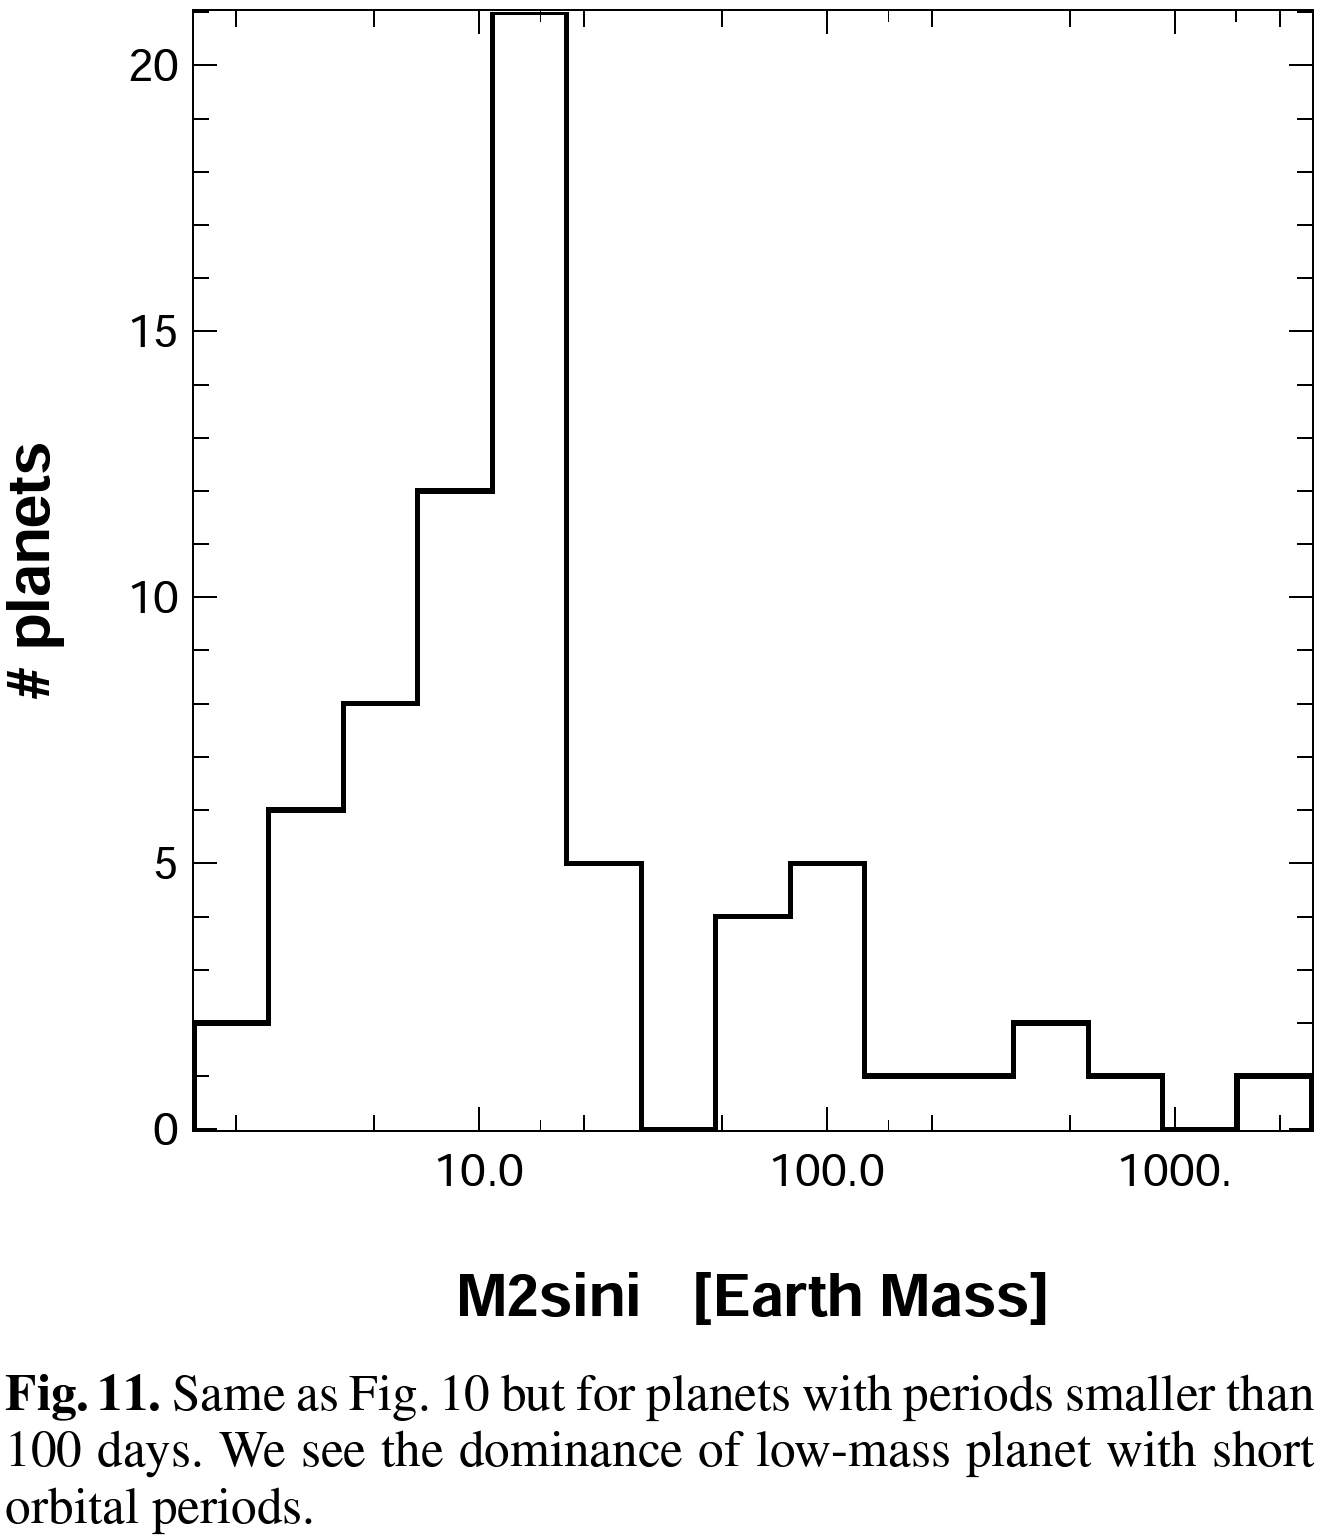
\includegraphics[trim={0cm 0 0 0},clip,height=0.45\textheight]{pvsMP100}\label{fig:pvsMP100}
\end{subfigure}
\end{figure} 

\begin{figure}[!ht]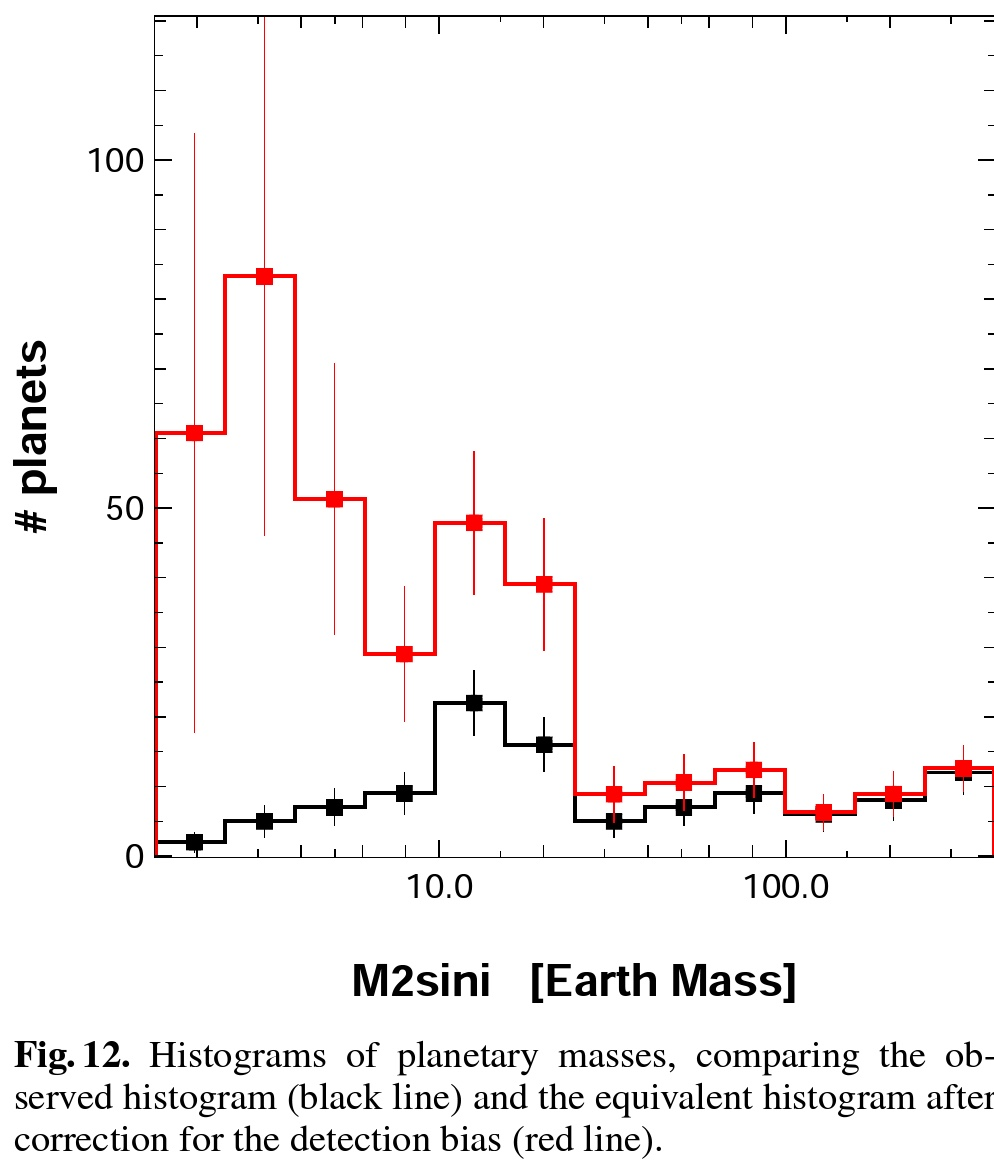
\includegraphics[trim={0cm 0cm 0 0},clip, keepaspectratio,height=0.45\textheight]{freqvsM}\label{fig:freqvsM}
\end{figure}

\end{frame}

\begin{wordonframe}{Distribuzione masse}
Gap nella distribuzione di massa attorno a $30\mearth{}$, popolazione di pianeti con massa minore di $10\mearth{}$ con $P<\SI{100}{\day}$, distribuzione piatta in $\log{M}$ nel range $30\mearth{}-4\mjupiter{}$.
\end{wordonframe}

\begin{frame}{Distribuzione periodi planetarii (a): RV, Mayor 11}
\begin{figure}[!ht]
\begin{subfigure}[b]{0.47\textwidth} \centering 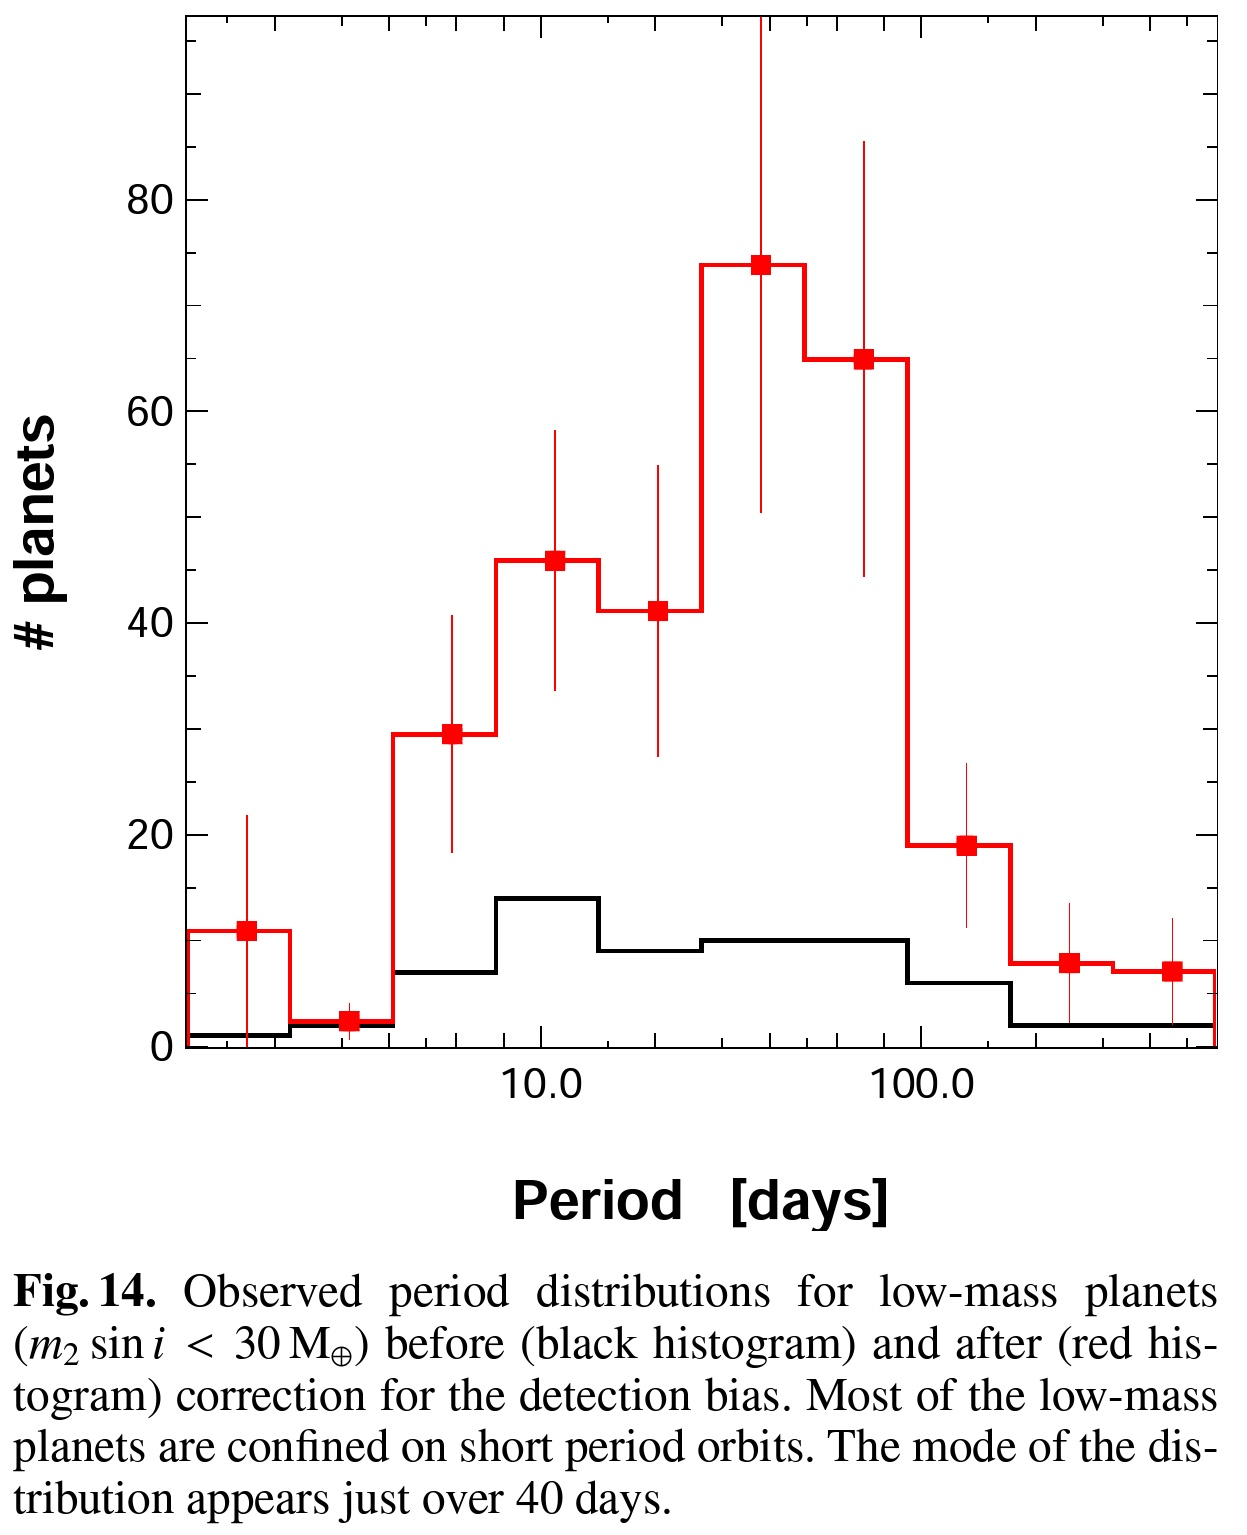
\includegraphics[trim={0cm 0 0 0},clip,width=0.99\textwidth]{freqvsPlowM}\label{fig:freqvsPlowM}\end{subfigure}
~
\begin{subfigure}[b]{0.47\textwidth} \centering 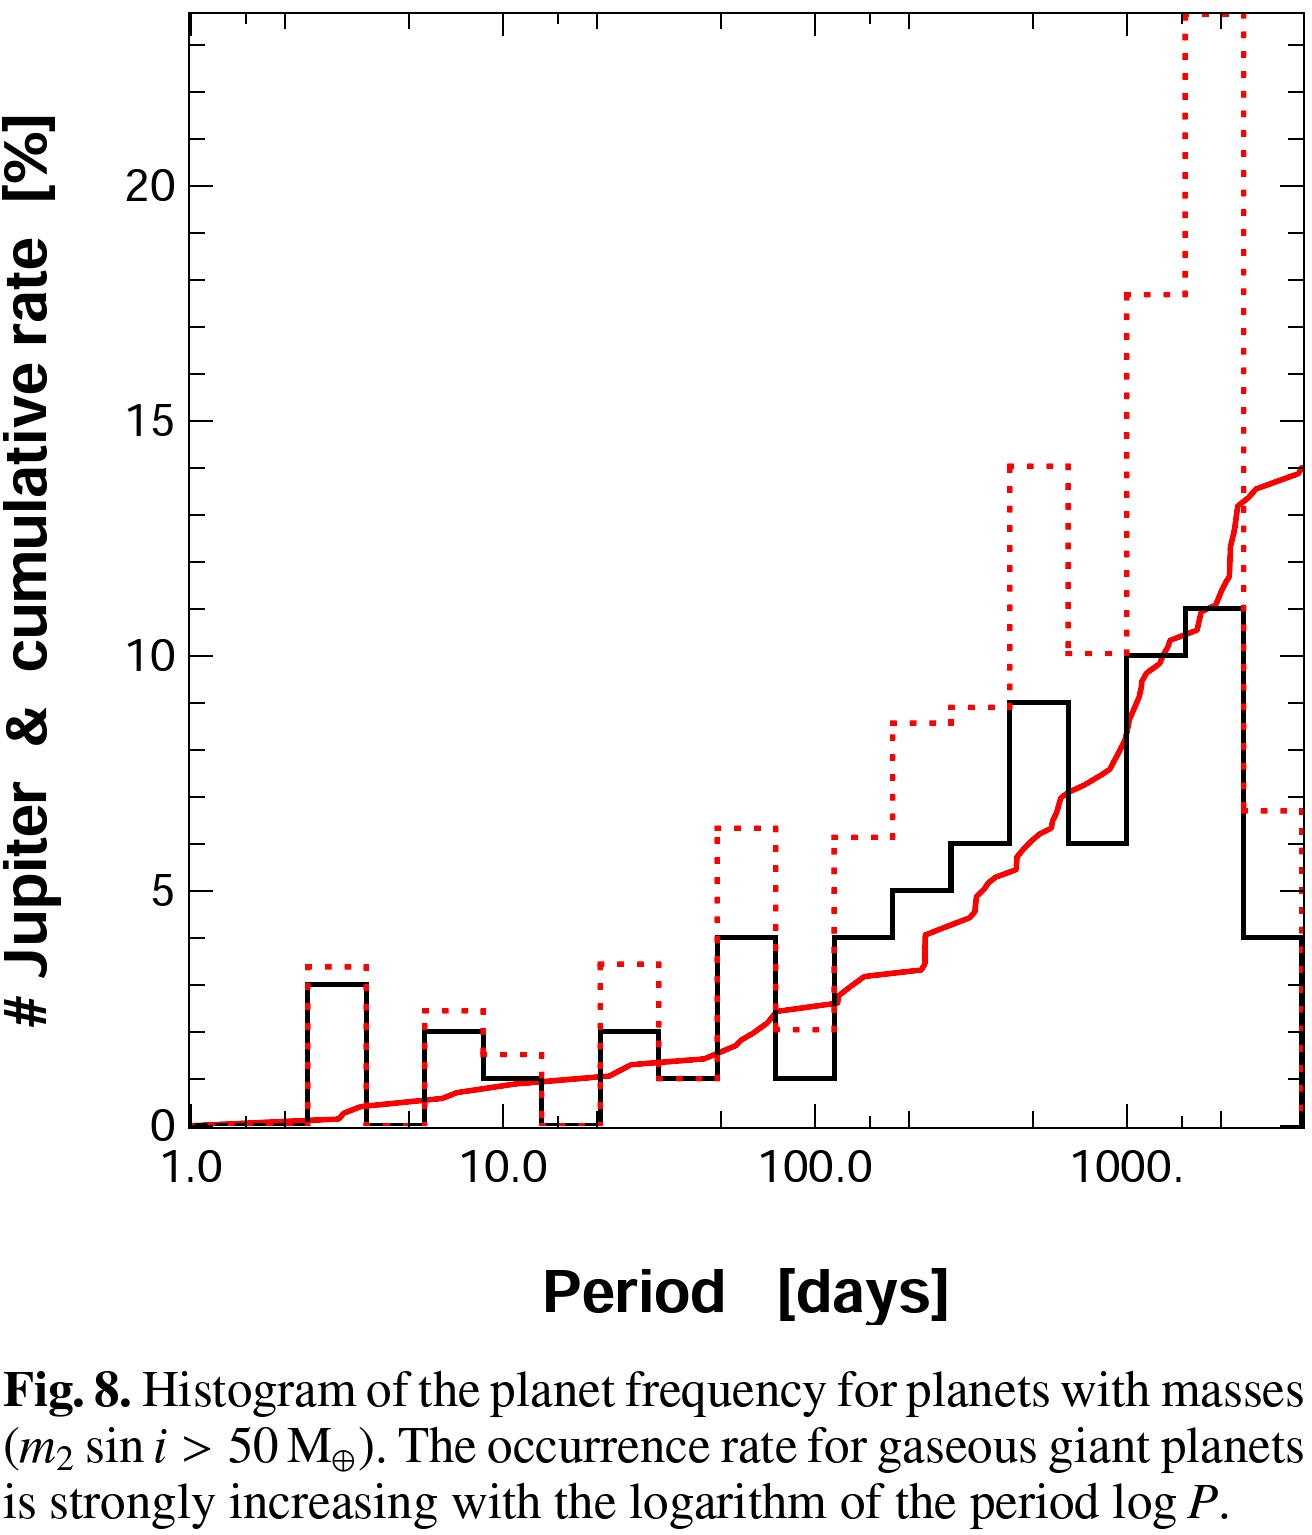
\includegraphics[trim={0cm 0 0 0},clip, height=0.5\textheight]{freqvsPgiant} \label{fig:freqvsPgiant} \end{subfigure}
\end{figure}
\end{frame}

\begin{wordonframe}{Distribuzione periodi}
I pianeti giganti sono raggruppati attorno a \SI{3}{\day}, possibile minimo entro \SI{100}{\day} e distribuzione che cresce rapidamente dopo \SI{100}{\day}.
Pianeti $M<30\mearth{}$ concentrati in \SIrange{10}{100}{\day}.
\end{wordonframe}

\begin{frame}{Caratteristiche orbitali: RV, Mayor 11}
\begin{figure}[!ht]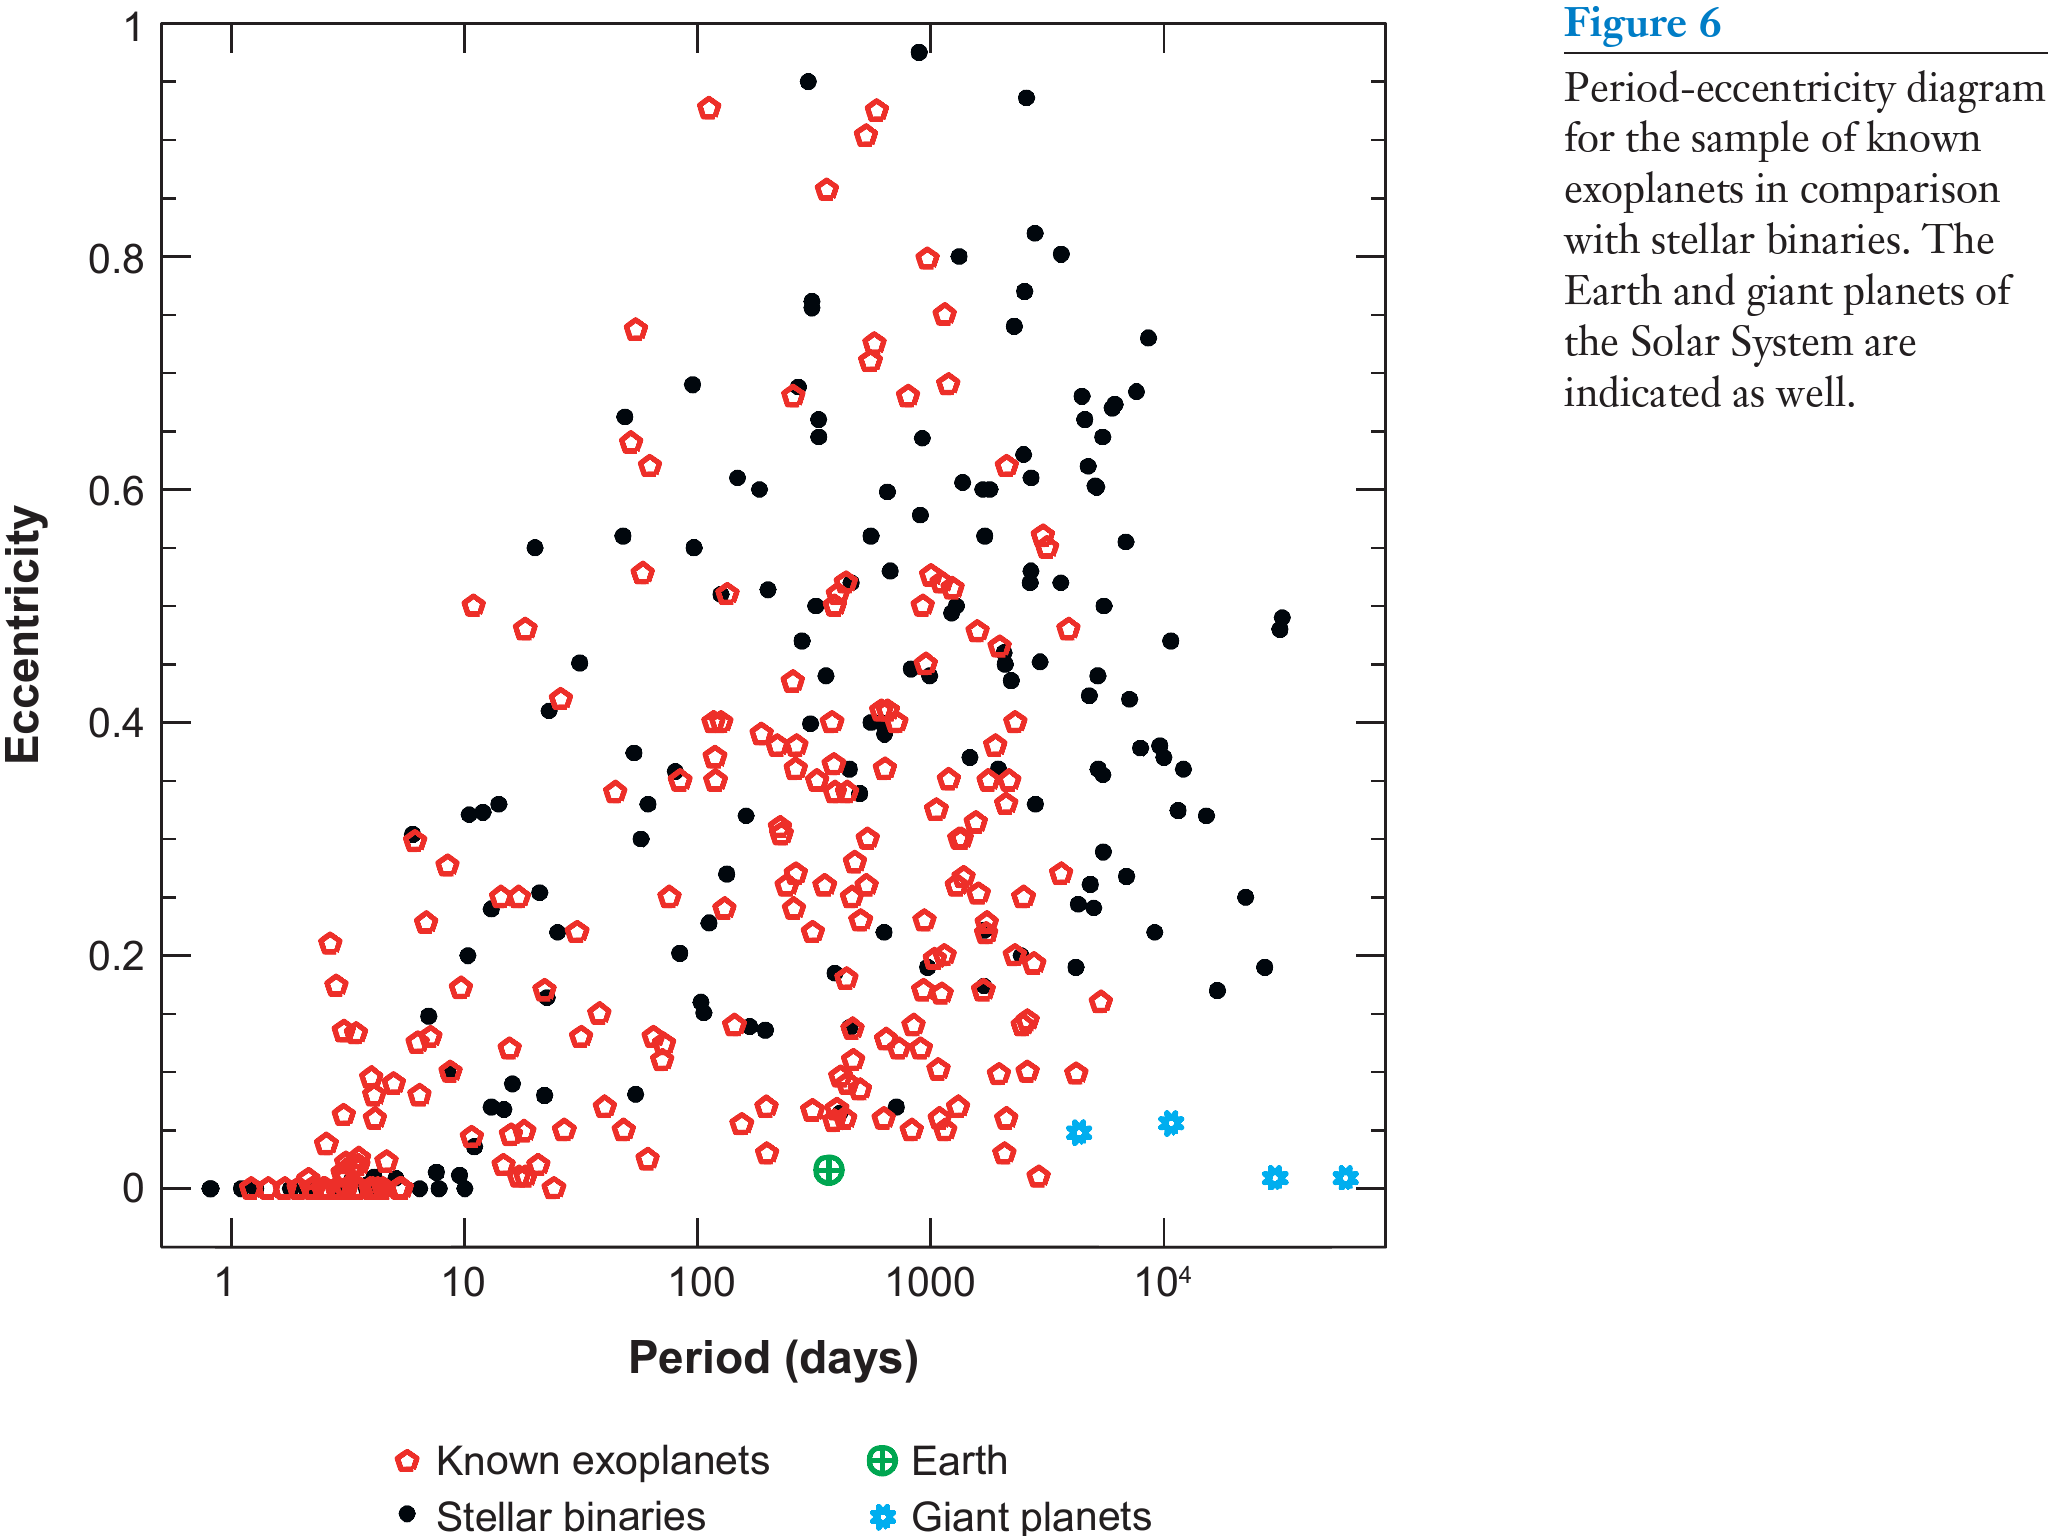
\includegraphics[trim={0cm 0cm 0 0},clip, keepaspectratio,width=0.5\textwidth]{eP}\label{fig:eP}\end{figure}
$\exv{e}\approx0.29$ - binary stars.

\begin{columns}[T]\begin{column}{0.5\textwidth}
Large scattering of e for gas giant (up to 0.93), up to $0.45$ for $M<30\mearth{}$.
\end{column} \begin{column}{0.5\textwidth}
\begin{equation*}
dN=S(x,\sigma_x)\,dx=\frac{x}{\sigma_x^2}\exp{-\frac{x^2}{2\sigma_x^2}} 
\end{equation*}
\end{column}  \end{columns}

\end{frame}

\begin{wordonframe}{Propriet\'a orbitali}
Fuori dalla regione di circolarizzazione mareali, $P=\SIrange{10}{30}{\day}$, ci sono comunque sistemi con piccola e (Sistema solare): evoluzione nel disco proto-planetario.
Sistemi con grande eccentricit\'a con $P=\SIrange{6}{10}{\day}$: influenza di compagno a grande periodo.
Planet-Planet scattering: upper part follow Rayleigh distribution.
\end{wordonframe}

\begin{frame}{Sistemi multipli e metallicit\'a}

\begin{figure}[!ht]
\begin{subfigure}[b]{0.47\textwidth} \centering 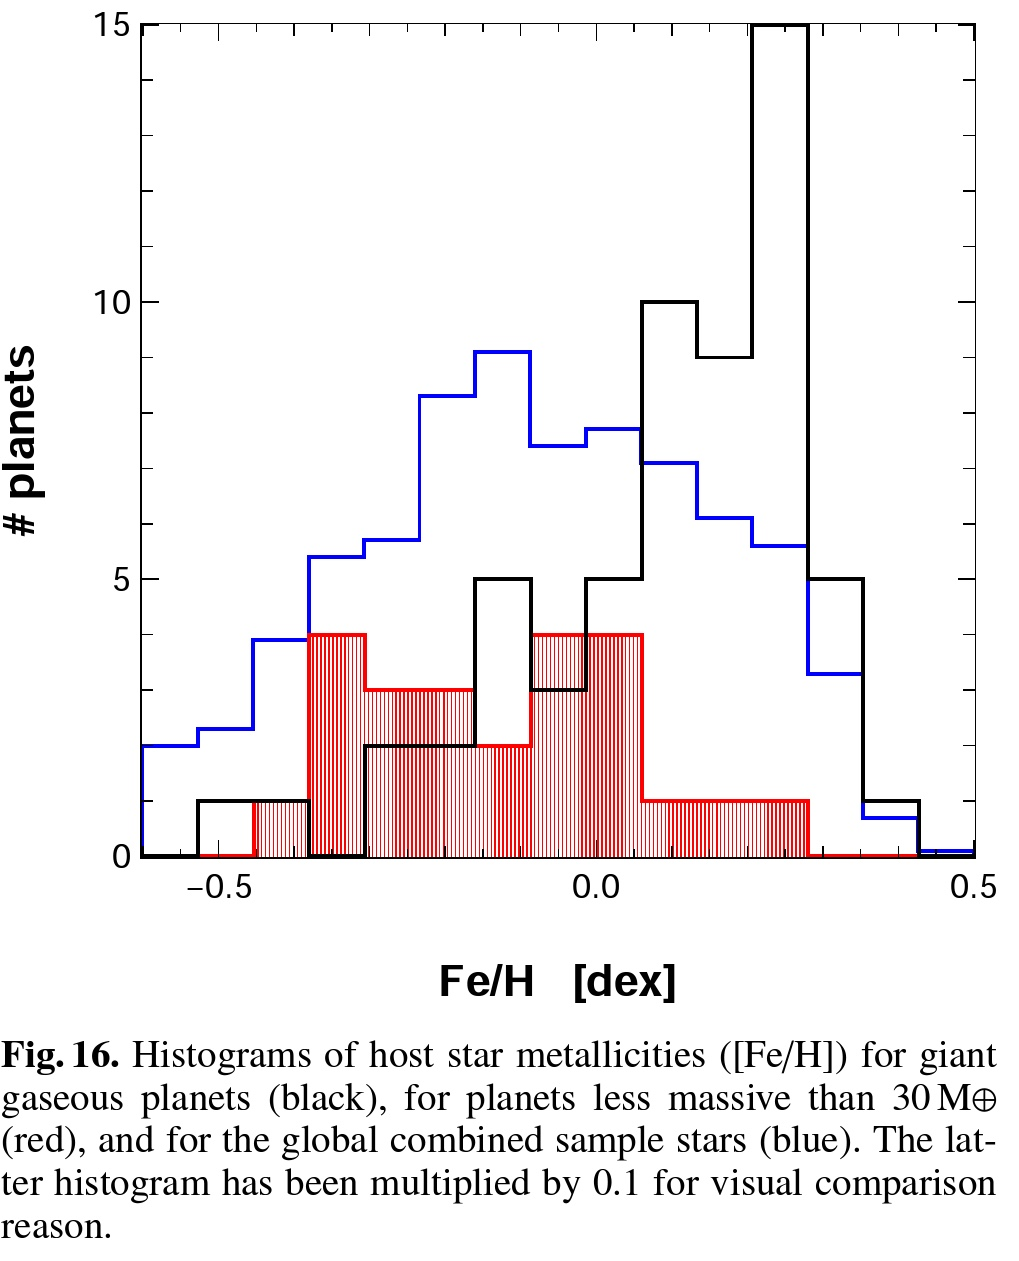
\includegraphics[trim={0cm 0 0 0},clip, height=0.45\textheight]{pvsFeH}\label{fig:pvsFeH} \end{subfigure}
~
\begin{subfigure}[b]{0.47\textwidth} \centering 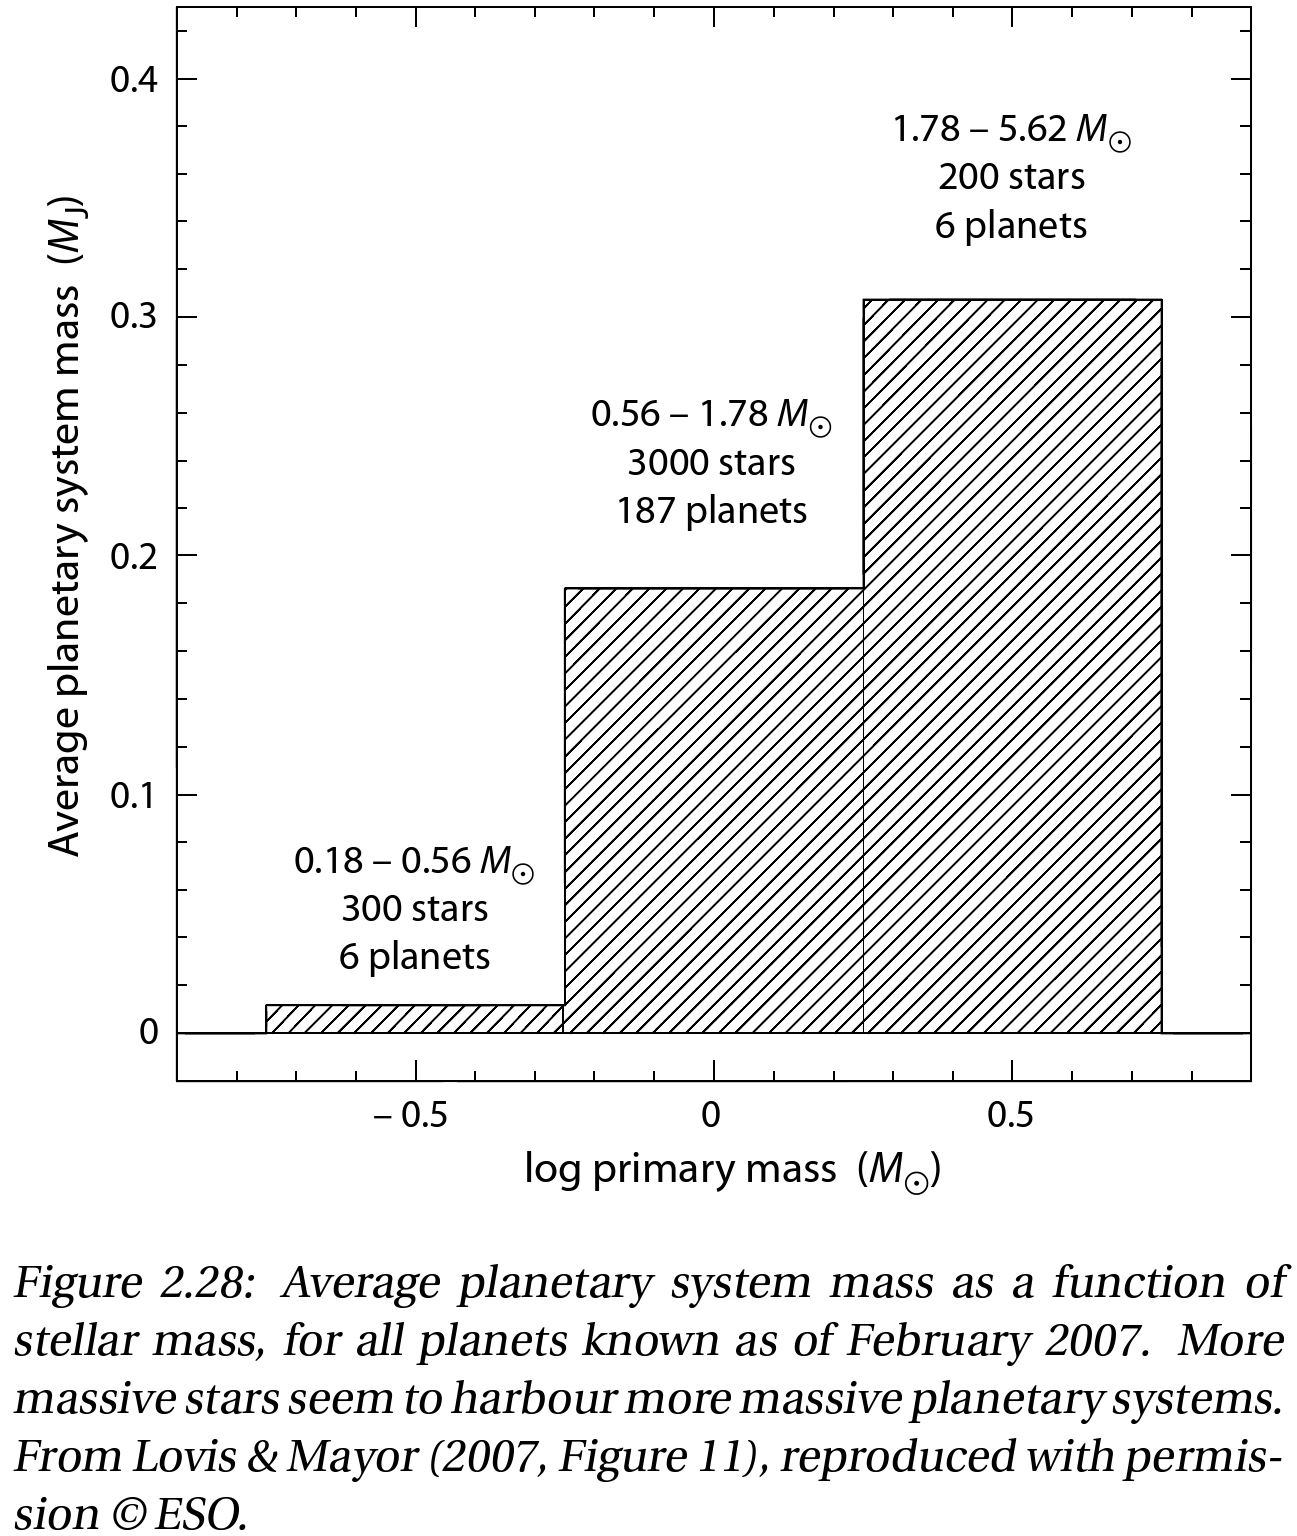
\includegraphics[trim={0cm 0 0 0},clip,height=0.45\textheight]{pMstar}\label{fig:pMstar}\end{subfigure}
\end{figure}
\begin{figure}[!ht]
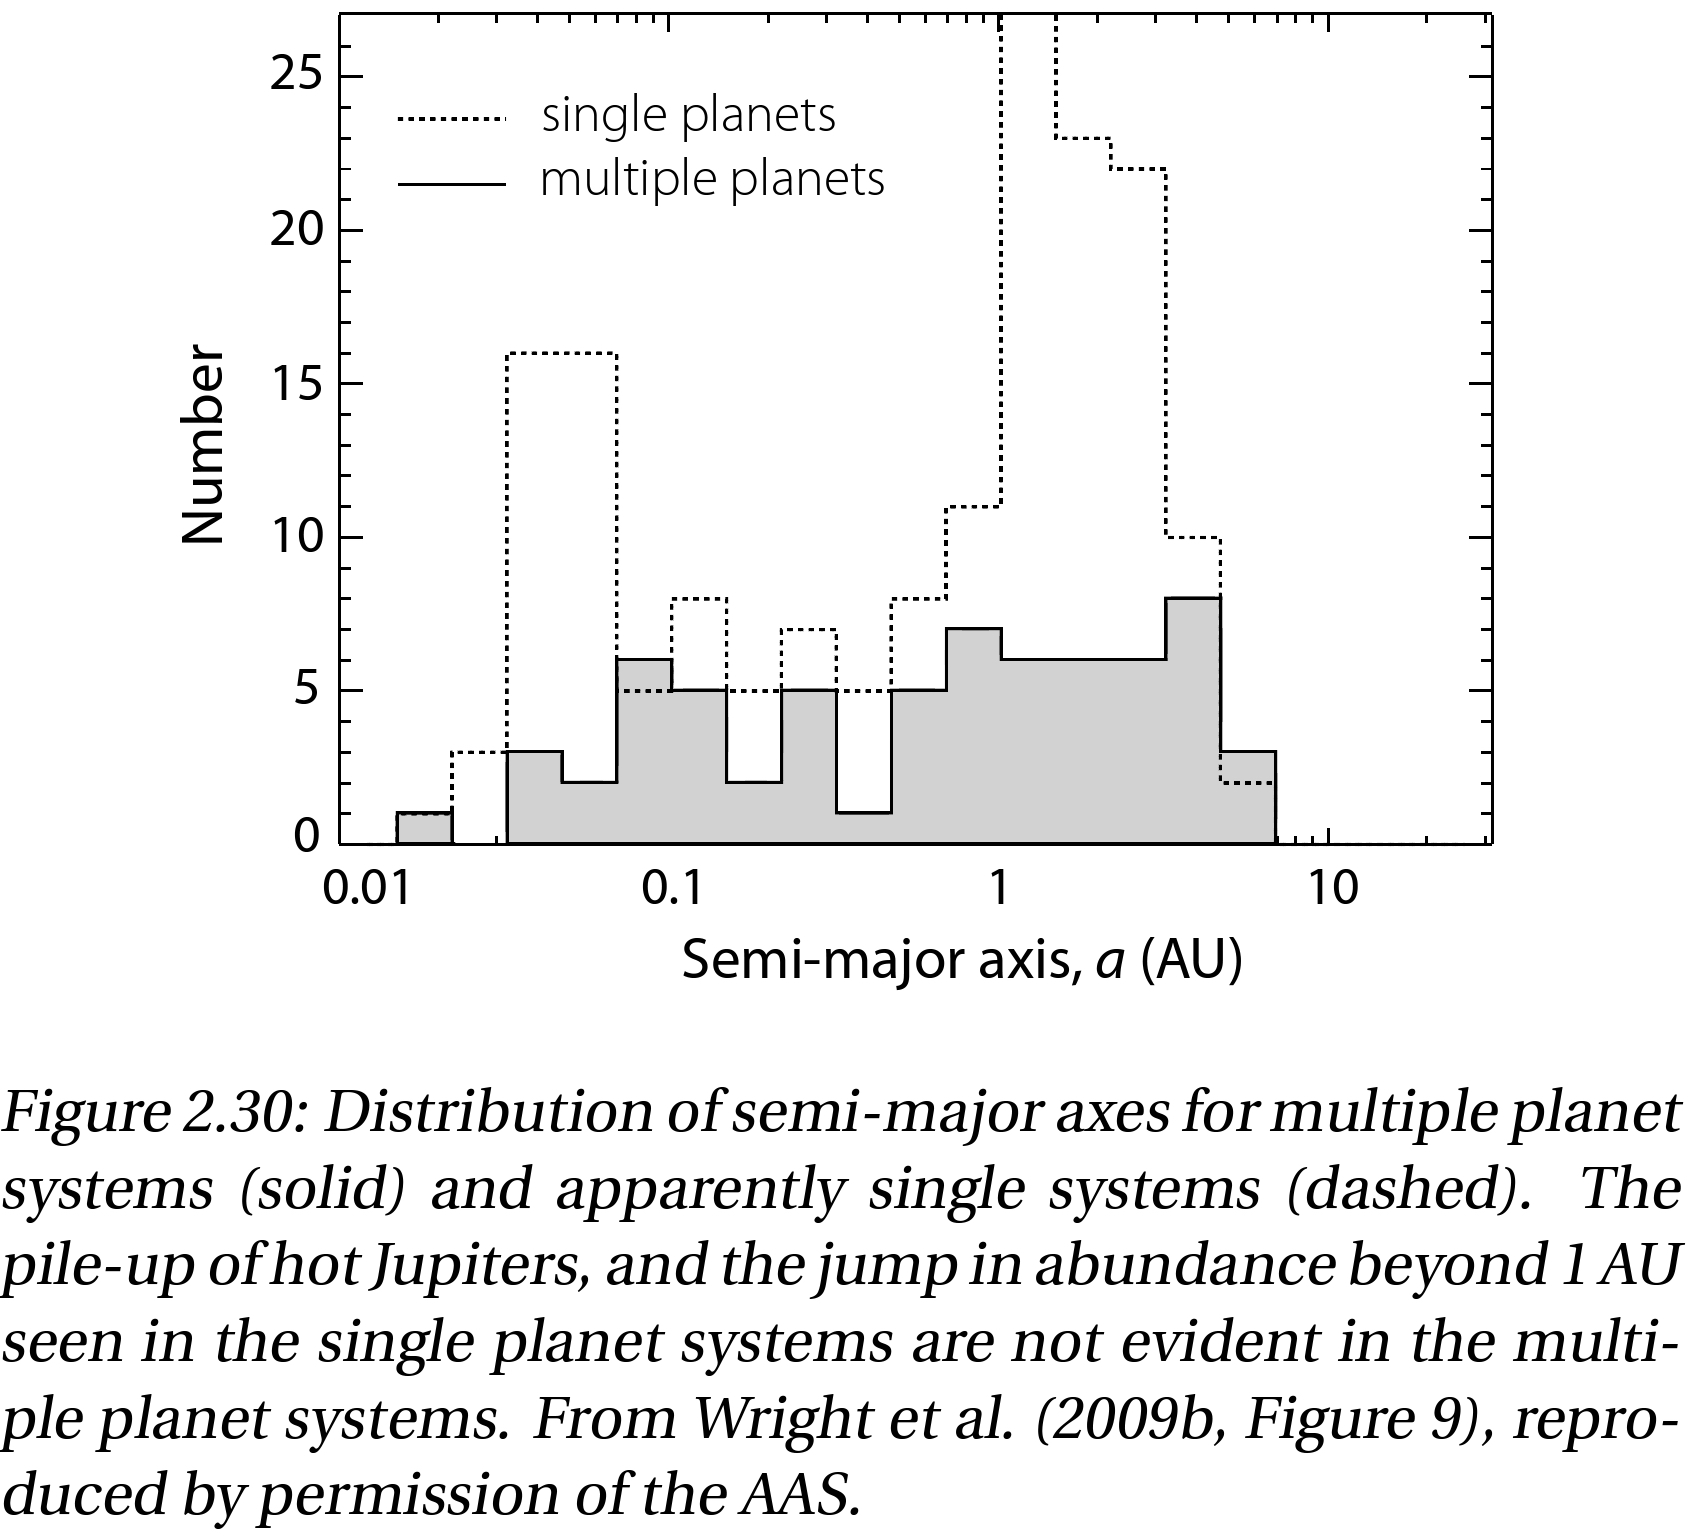
\includegraphics[trim={0cm 0cm 0 0},clip, keepaspectratio,height=0.45\textheight]{a-single-multi}\label{fig:a-single-multi}\end{figure}
\end{frame}

\begin{wordonframe}{Correlazione con caratteristiche stellari e sistemi multipli}
La frequenza dei pianeti giganti aumenta con la metallicit\'a stellare (Santos 04, Fischer Valenti 05); inoltre cresce nel range $1-2\msun{}$.
I sistemi multipli possono essere classificati in maniera non esclusiva secondo il numero di pianeti giganti, la presenza di MMR, secondo l'importanza delle interazioni pianeta-pianeta, la presenza di pianeti sub-gioviani.
La distribuzione dei periodi nei sistemi multipli mostra accumulo meno pronunciato a \SI{3}{\day}, e \SI{1}{\astronomicalunit}
\end{wordonframe}


\section{Properties of transit exoplanets}\linkdest{exoT}

\begin{frame}{Distribuzione raggio planetario}
\begin{columns}[T] \begin{column}{0.5\textwidth}
\begin{figure}[!ht]
\centering 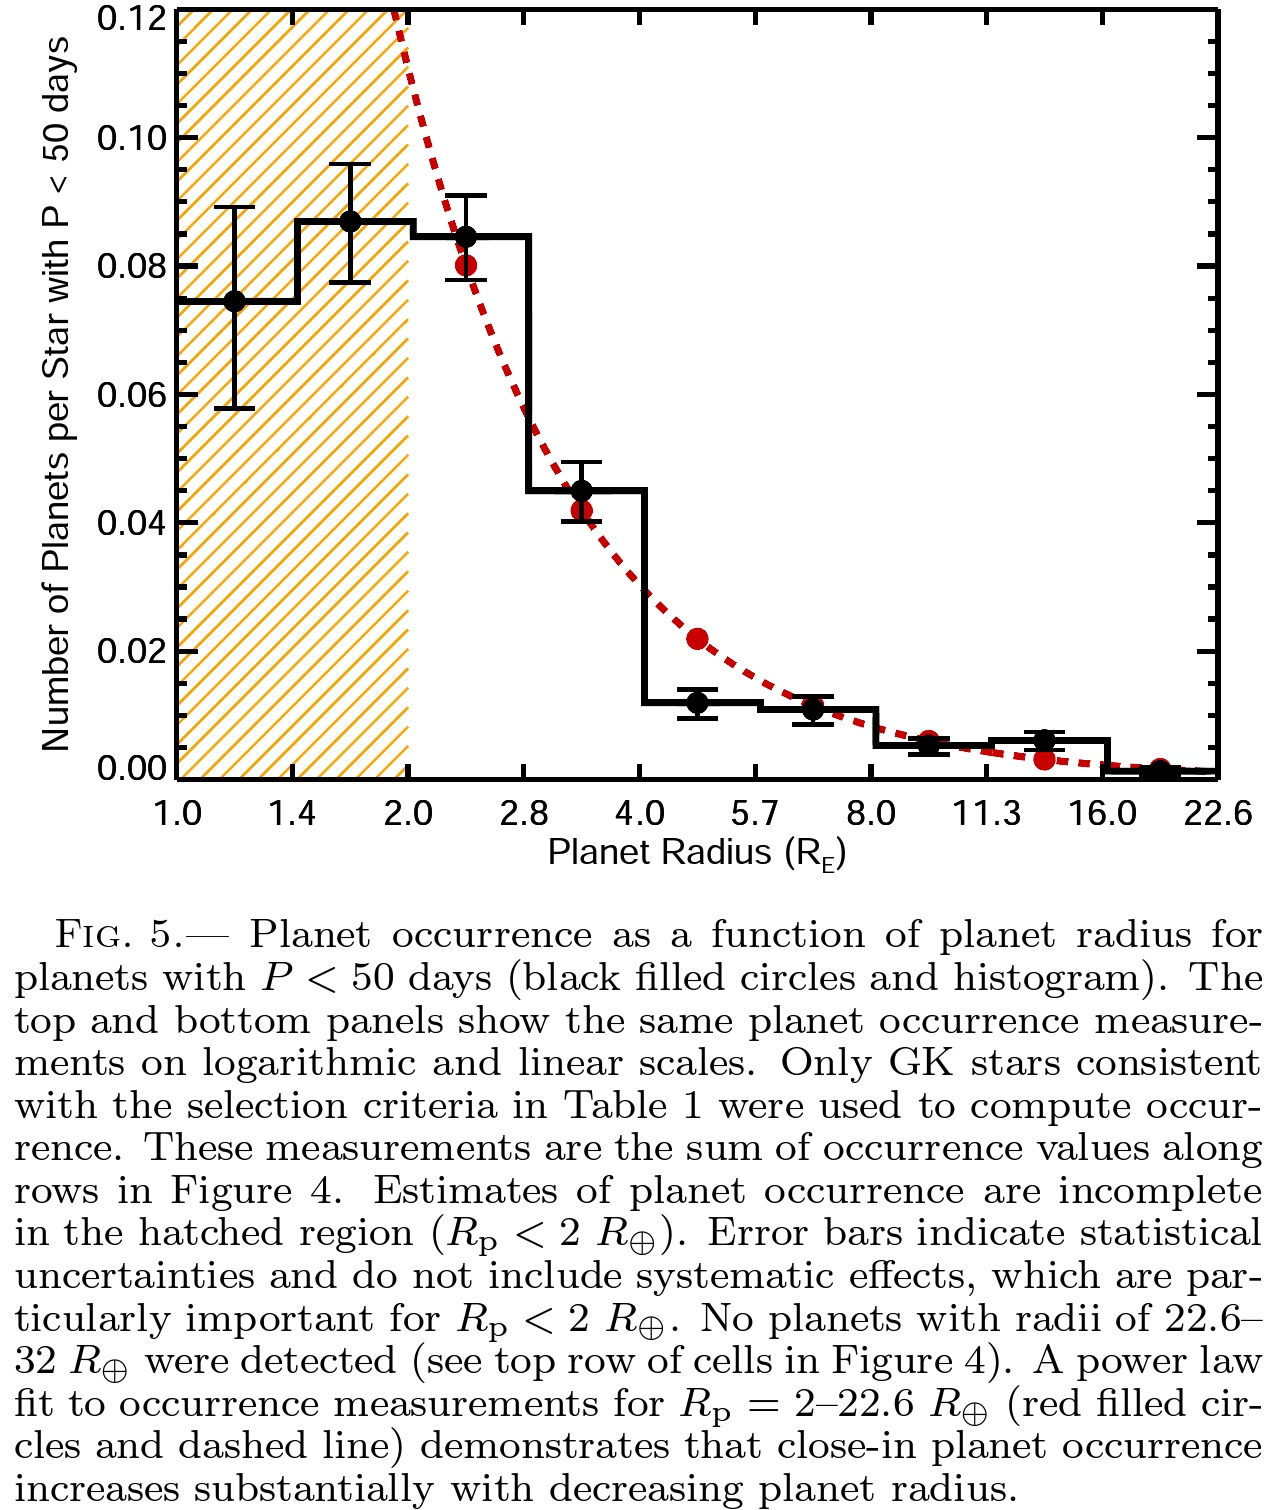
\includegraphics[trim={0cm 23cm 0 0},clip,height=0.22\textheight]{freqvsRpl50d}\label{fig:freqvsRpl50d}\end{figure}%
\begin{figure}[!ht]\centering 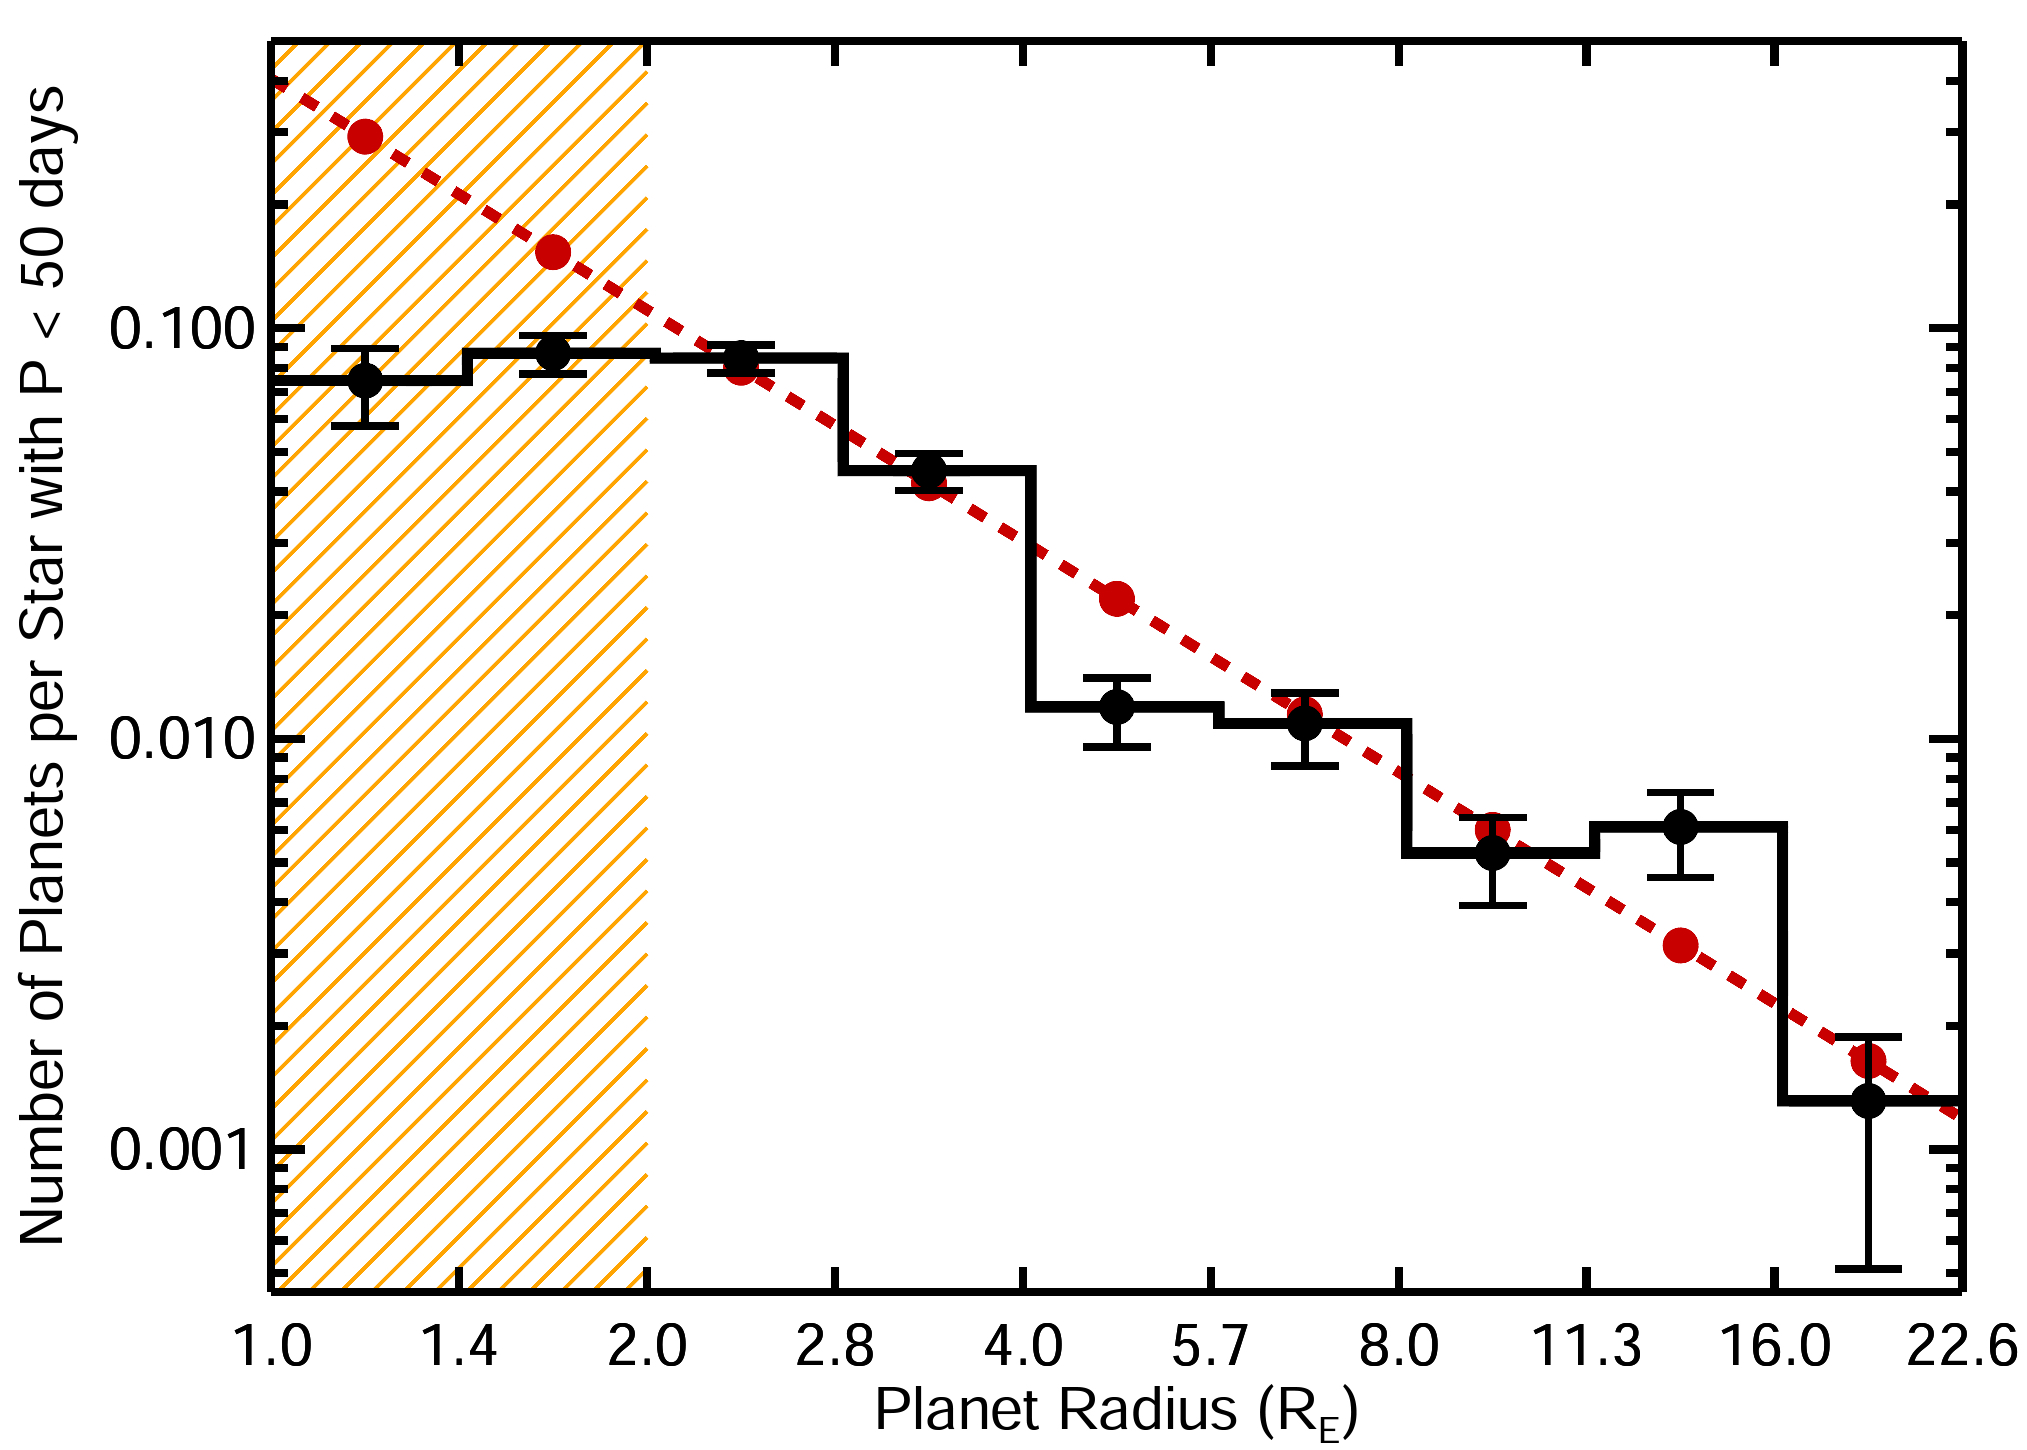
\includegraphics[trim={0cm 1cm 0 0},clip, height=0.22\textheight]{freqvsRpl50dl} \label{fig:freqvsRpl50dl}
\end{figure}%
\begin{figure}[!ht]\centering 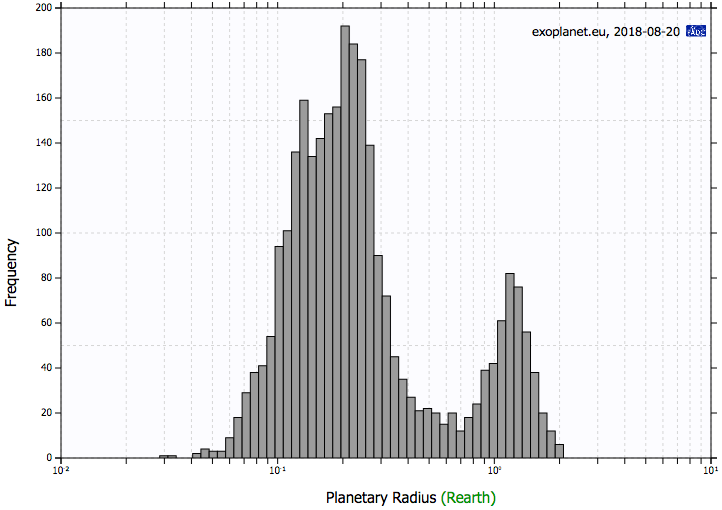
\includegraphics[trim={0cm 0cm 0 0},clip, height=0.25\textheight]{freqR-T} \label{fig:freqR-T}
\end{figure}%
\end{column} \begin{column}{0.5\textwidth}
\cite{howard2012planet}: $P<\SI{50}{\day}$, $R=\numrange{2}{22.7}\rearth{}$
\begin{align*}
&\TDy{\log{R}}{f(R)}=K_RR\expy{\alpha}\\
&\alpha=-1.92\pm0.11,\ K_R=2.9_{-0.4}^{0.5}
\end{align*}
\end{column}  \end{columns}
\end{frame}

\begin{wordonframe}{Relazione massa-raggio: equazione di stato, composizione e evaporazione}
Equazione di stato: $P\propto\rho\expy{\gamma}$, $\gamma=1+\frac{1}{n}$; una relazione con n maggiore \'e causata da materia meno comprimibile.
\end{wordonframe}

\begin{frame}{Distribuzione periodo orbitale}
\begin{figure}[!ht]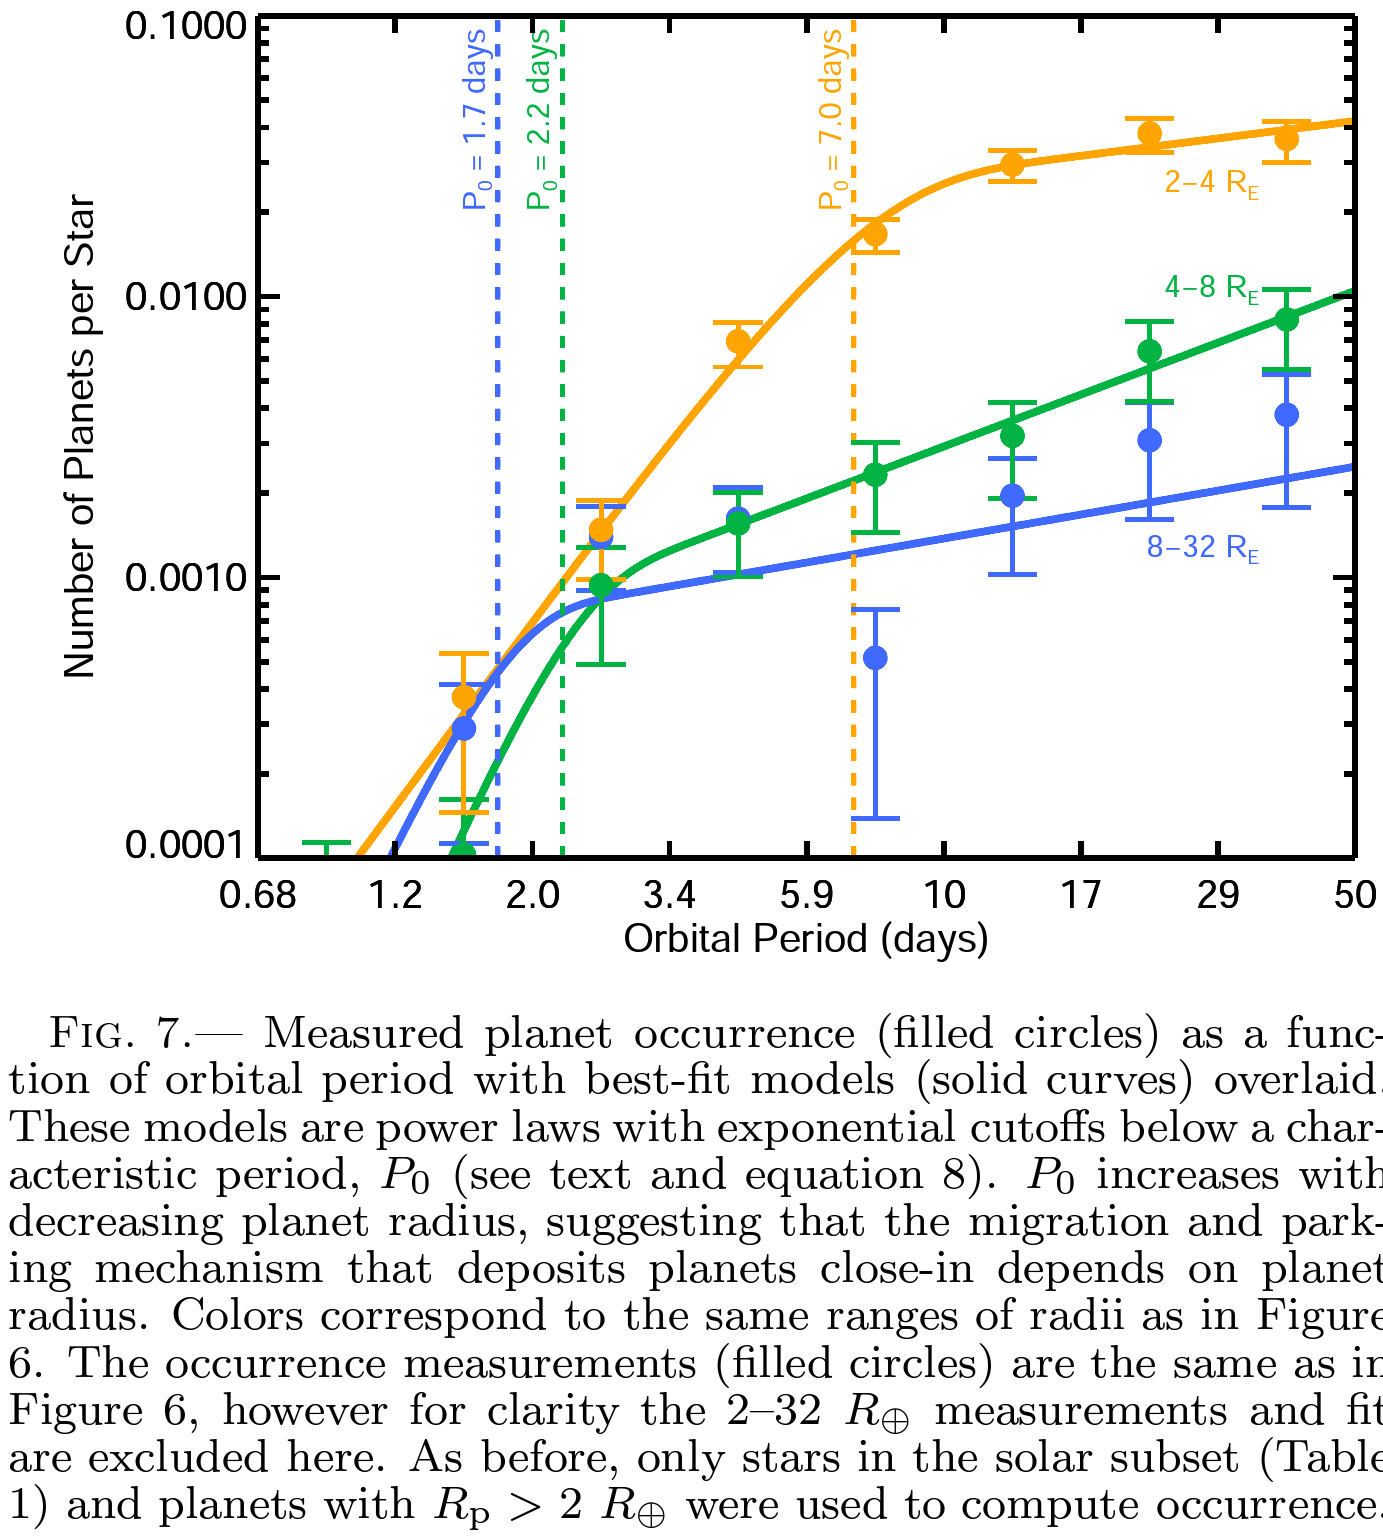
\includegraphics[trim={0cm 0cm 0 0},clip, keepaspectratio,height=0.5\textheight]{freqperstarvsPanfit}\label{fig:freqperstarvsPanfit}\end{figure}

\end{frame}

\section{Orbital evolution}

\subsection{Propriet\'a orbitali}

\subsection{Hot Jupiters due to tidal circularization}

\begin{frame}{Planet-Planet scattering}
Scattering in eccentric close-in orbit. Tidal circularization: limit distance twice the Roche limit.
\end{frame}

\begin{wordonframe}{Tidal circularization}
During circularization angular momentum $\propto \sqrt{GMa(1-e^2)}$: for $e\approx1$: $a_f=a_i(1-e^2)\approx2a_{peri}$.

$R_p=0.462a_R(\frac{M_p}{M_*})\expy{\frac{1}{3}}$ 
\end{wordonframe}
